\chapter{root systems}
\section{abstract root systems} \label{7.1}
\begin{itemize}
	\item \textbf{def.:} a \textbf{root system} $(E, R)$ is a finite-dimensional vector space $E = \mathrm{span}(R)$, with a finite collection of non-zero vectors $R$, and an inner product $\braket{\cdot, \cdot}$, and,
	\begin{enumerate}
		\item $E = \mathrm{span}(R)$,
		
		\item if $\alpha \in R$, then $c \alpha \in R \iff c = \pm 1$,
		
		\item if $\alpha, \beta \in R$, then $s_\alpha \ket{\beta} \in R$, where $s_\alpha = 1 - 2 \frac{\ket{\alpha} \bra{\alpha}}{\braket{\alpha, \alpha}}$,
		
		\item for all $\alpha, \beta \in R$, $2 \frac{\braket{\alpha, \beta}}{\braket{\alpha, \alpha}} \in \mathbb{Z}$.
	\end{enumerate}
	$\dim E$ is called the \textbf{rank} of the system, elements in $R$ are called \textbf{roots}.
	
	\item \textbf{def.:} the \textbf{Weyl group}, $W$, of $R$ is the finite subgroup of the orthogonal group of $E$ generated by $s_\alpha, \forall \alpha \in R$.
	
	\noindent\rule[0.5ex]{\linewidth}{0.5pt} % horizontal line
	
	\item \textbf{def.:} $(E, R)$ and $(F, S)$ are two root systems, then $(E \oplus F, R \cup S)$ is a root system, and $R \cup S$ is called the \textbf{direct sum} of $R$ and $S$.
	
	(it is easy to see the direct sum root system satisfies the def. of root systems)
	
	\item \textbf{def.:} a root system is called \textbf{reducible} if there exists an orthogonal decomposition $E = E_2 \oplus E_2$ with $E_1 \perp E_2$ and $\dim E_i > 0$, and every root is either in $E_1$ or $E_2$.
	\begin{itemize}
		\item the root system of a semisimple Lie algebra is irreducible $\iff$ the semisimple Lie algebra is simple (见 section \ref{6.6} 最后一个定理).
	\end{itemize}
	
	\item \textbf{def.:} an \textbf{isomorphism} is a linear map that \textbf{preserves the reflection}, not the inner product,
	\begin{equation}
		A : E \rightarrow F \quad \text{s.t.} \quad A s_\alpha \ket{\beta} = s_{A \alpha} \ket{A \beta}
	\end{equation}
	
	\noindent\rule[0.5ex]{\linewidth}{0.5pt} % horizontal line
	
	\item 对于 $\braket{\beta, \beta} \leq \braket{\alpha, \alpha}$, 且 $\beta \cancel{\propto} \alpha$, 根 $\alpha, \beta$ 之间可能的关系如下,
	\begin{itemize}
		\item $\beta \perp \alpha$.
		
		\item or, $\braket{\alpha, \alpha} = 1, 2, 3 \braket{\beta, \beta}$ (图中没有画出 $\beta \mapsto - \beta$ 的情况, 那时夹角是图中夹角的补角).
		
		\begin{figure}[H]
			\centering
			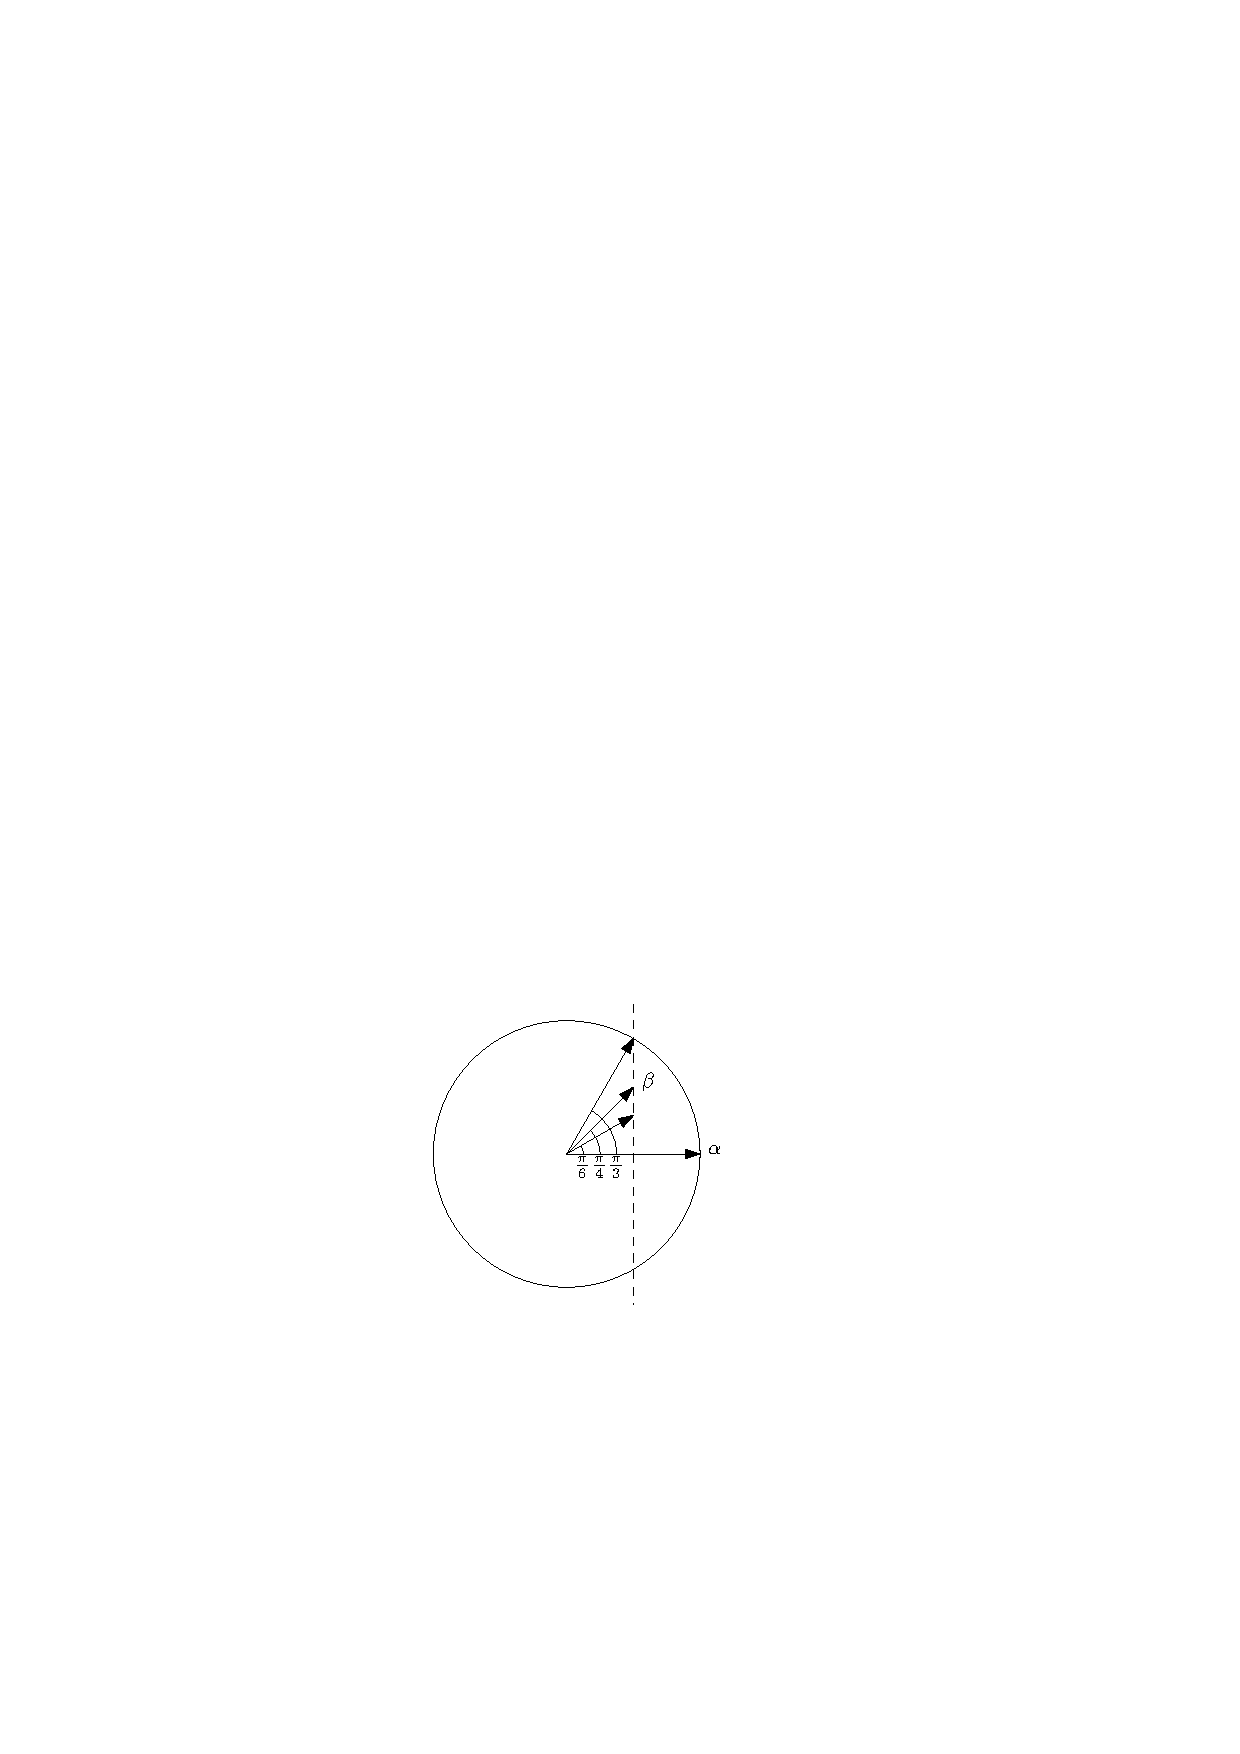
\includegraphics[scale=1]{figures/the basic acute angles and length ratios.pdf}
		\end{figure}
	\end{itemize}
	
	\item 如果根 $\alpha, \beta$ 之间夹锐角, 那么 $\pm (\alpha - \beta)$ 也是根;如果夹钝角, 那么 $\pm (\alpha + \beta)$ 也是根.
	
	\begin{tcolorbox}[title=proof:]
		假设 $\braket{\alpha, \alpha} \geq \braket{\beta, \beta}$, 考虑夹锐角的情况, 此时, $\beta - \alpha = s_\alpha \ket{\beta}$;对于夹钝角的情况, 令 $\beta' = - \beta$ 即可.
	\end{tcolorbox}
\end{itemize}

\section{rank-two systems}
\begin{itemize}
	\item if rank is one, the roots are $R = \{- \alpha, \alpha\}$.
	
	\item \textbf{every rank-two system} is isomorphic to one of the systems below,
	
	\begin{figure}[H]
		\centering
		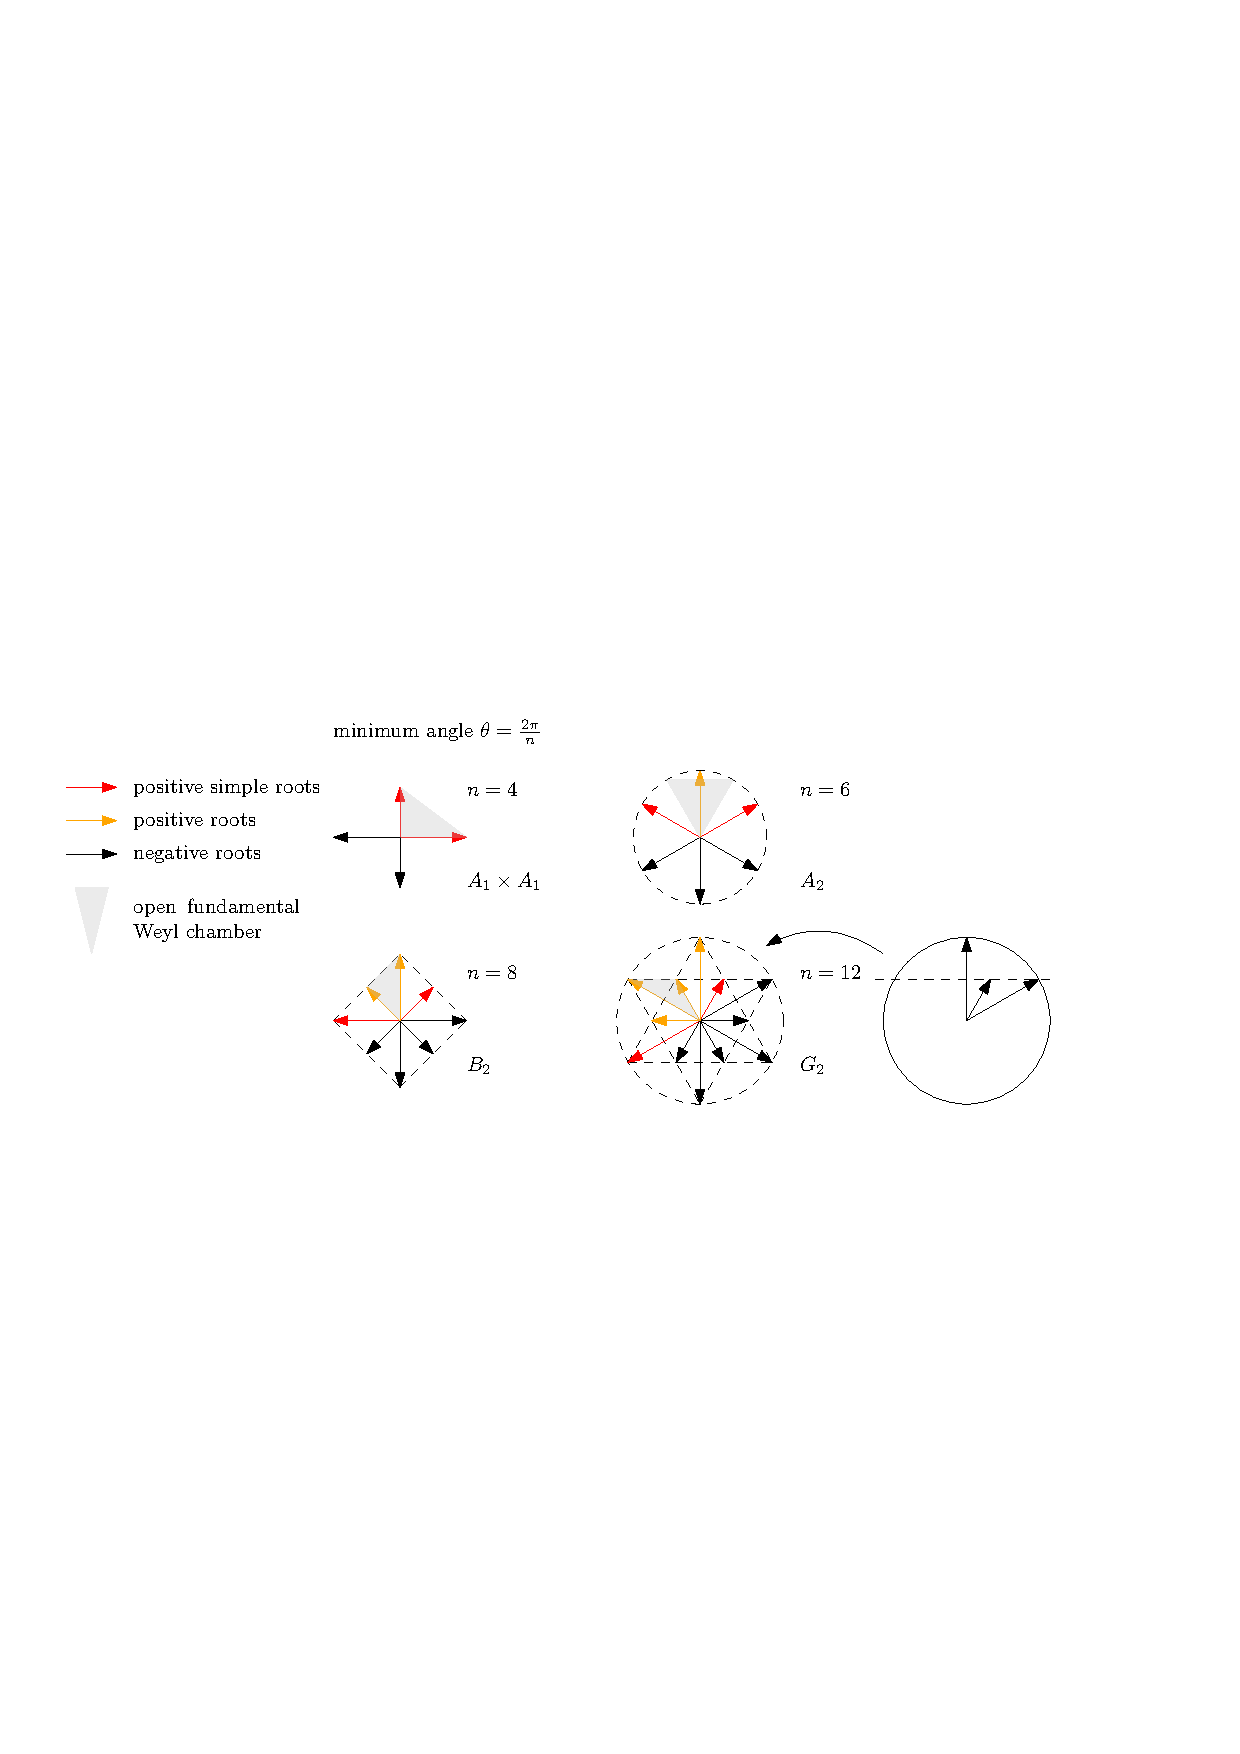
\includegraphics[scale=1]{figures/the rank-two root systems.pdf}
	\end{figure}
	
	分别考虑两个根之间最小夹角为 $\frac{\pi}{6}, \frac{\pi}{4}, \frac{\pi}{3}, \frac{\pi}{2}$ 的情况, 然后使用 $s_\alpha \ket{\beta}$ 生成整个 $R$.
	
	for positive simple roots, positive roots, negative roots and Weyl chambers, see section \ref{7.4}.
	
	\item the \textbf{Weyl group} of a rank-two root system, $R$, with minimum angle $\theta = \frac{2 \pi}{n}$ is the symmetry group of a regular $\frac{n}{2}$-gon (正 $\frac{n}{2}$ 边形).
	\begin{itemize}
		\item 群元素包括 $\frac{n}{2}$ 个镜面反射和 $2 \theta$ 转动.
	\end{itemize}
\end{itemize}

\section{duality}
\begin{itemize}
	\item \textbf{def.:} for a root $\alpha \in R$ in a root system $(E, R)$, its \textbf{coroot} is,
	\begin{equation}
		H_\alpha = 2 \frac{\alpha}{\braket{\alpha, \alpha}} \quad \text{with} \quad \begin{dcases}
			s_{H_\alpha} = s_\alpha \\
			\frac{\braket{H_\alpha, H_\beta}}{\braket{H_{\mathcolor{red}{\alpha}}, H_{\mathcolor{red}{\alpha}}}} = \frac{\braket{\alpha, \beta}}{\braket{\mathcolor{red}{\beta}, \mathcolor{red}{\beta}}}
		\end{dcases}
	\end{equation}
	and the \textbf{dual root system} to $R$ is $R^\vee = \{H_\alpha | \alpha \in R\}$.
	\begin{itemize}
		\item $R^\vee$ is also a root system, with the same Weyl group as $R$ (because $s_{H_\alpha} = s_\alpha$).
		
		\item $H_{H_\alpha} = \alpha$ and $(R^\vee)^\vee = R$.
		
		\item note that although $H_{s_\alpha \ket{\beta}} = s_{H_\alpha} \ket{H_\beta}$, the map $H$ is not linear, so $R^\vee$ and $R$ are not necessarily isomorphic to each other.
	\end{itemize}
\end{itemize}

\section{bases and Weyl chambers} \label{7.4}
\begin{itemize}
	\item \textbf{def.:} for a root system $(E, R)$, a subset $\Delta \subset R$ is called a \textbf{base} if,
	\begin{enumerate}
		\item $\Delta$ is a basis of $E$,
		
		\item each root $\alpha \in R$ can be expressed as a linear combination of basis vectors in $\Delta$ with non-negative (positive roots, $R^+$) or non-positive (negative roots, $R^-$) integer coefficients, $R = R^+ \cup R^-$.
	\end{enumerate}
	elements in $\Delta$ are called \textbf{positive simple roots}.
	
	\item $\alpha \neq \beta \in \Delta$, then $\braket{\alpha, \beta} \leq 0$.
	
	\begin{tcolorbox}[title=proof:]
		如果 $\alpha, \beta$ 之间夹锐角, 那么 $\pm (\alpha - \beta)$ 也是根, 不满足系数同时非负 (或非正) 的要求.
	\end{tcolorbox}
	
	\item for a root system $(E, R)$, there exists a hyperplane $V$ through the origin in $E$, s.t. $V$ does not contain any root.
	
	\begin{tcolorbox}[title=proof:]
		考虑一个向量 $H \in E$, 它不在任何一个垂直于某个根向量的超平面 (这样的超平面有限多, 所以 $H$ 存在) 上, 那么 $V \perp H$ 就是我们要找的超平面.
	\end{tcolorbox}
	
	\item \textbf{def.:} choose one side of $V$ to be $R^+$, the other side to be $R^-$, an element $\alpha \in R^+$ is \textbf{decomposable} if $\alpha = \beta + \gamma$ for some $\beta, \gamma \in R^+$, otherwise, $\alpha$ is \textbf{indecomposable}.
	
	\item the indecomposable roots in $R^+$ form the base $\Delta$, and $\Delta$ exists.
	
	\begin{tcolorbox}[title=proof:]
		let $\Delta$ denote the set of indecomposable elements in $R^+$, now we will prove $\Delta$ is the base:
		\begin{itemize}
			\item every $\alpha \in R^+$ can be expressed as a linear combination of elements in $\Delta$ with non-negative integer coefficients.
			
			\noindent\rule[0.5ex]{\linewidth}{0.5pt} % horizontal line
			
			\textbf{proof:}
			
			\begin{itemize}
				\item 考虑 $H \perp V$, 且 $\braket{\alpha, H} > 0, \forall \alpha \in R^+$.
				
				\item 考虑 $\Delta'$ 是不能表示成 $\Delta$ 的元素的非负整数系数的线性叠加的 $R^+$ 元素的集合, 那么一定有 $\Delta' \cap \Delta = \emptyset$.
				
				\item 考虑 $\alpha \in \Delta'$ 且 $\braket{\alpha, H}$ 是 $\Delta'$ 中元素里最小的, 而且 $\alpha = \beta_1 + \beta_2$ (且 $\beta_1, \beta_2 \in R^+$), 那么 $\beta_1, \beta_2$ 至少有一个是 $\Delta'$ 的元素, 但是 $\braket{\alpha, H} = \braket{\beta_1, H} + \braket{\beta_2, H}$ 这与 $\braket{\alpha, H}$ 最小矛盾.
				
				\item 可见 $\beta_1, \beta_2 \notin \Delta'$, $\alpha$ 一定可以表示为 $\Delta$ 的元素的...的线性叠加.
			\end{itemize}
			
			\noindent\rule[0.5ex]{\linewidth}{0.5pt} % horizontal line
			
			\item elements in $\Delta$ are linearly independent.
			
			\noindent\rule[0.5ex]{\linewidth}{0.5pt} % horizontal line
			
			\textbf{proof:}
			
			如果,
			\begin{equation}
				\sum_{\alpha \in \Delta} c'_\alpha \alpha = 0 \Longrightarrow \sum_\alpha c_\alpha \alpha = \sum_\beta d_\beta \beta = u \in R^+
			\end{equation}
			其中 $c_\alpha \geq 0, - d_\beta < 0$ 分别是 $\{c'_\alpha\}$ 中非负和负的系数, 等号两边对 $\Delta$ 的两个无交集的子集求和.
			
			考虑,
			\begin{equation}
				\braket{u, u} = \braket{\sum_\alpha c_\alpha \alpha, \sum_\beta d_\beta \beta} = \sum_{\alpha, \beta} c_\alpha d_\beta \braket{\alpha, \beta}
			\end{equation}
			但是, 对于 $\alpha \neq \beta \in \Delta$, 一定有 $\braket{\alpha, \beta} \leq 0$, 所以 $\braket{u, u} = 0$, 即 $u = 0$, 这与 $\alpha \in R^+$ 矛盾.
			
			\noindent\rule[0.5ex]{\linewidth}{0.5pt} % horizontal line
			
			\textbf{proof of $\boldsymbol{\braket{\alpha, \beta} \leq 0, \forall \alpha \neq \beta \in \Delta}$:}
			
			如果 $\alpha, \beta$ 呈锐角, 那么 $\pm (\alpha - \beta)$ 也是根, 且其中一个属于 $R^+$, 比如 $\alpha - \beta \in R^+$, 那么 $\alpha = (\alpha - \beta) + \beta$, 与 indecomposable 矛盾.
			
			\noindent\rule[0.5ex]{\linewidth}{0.5pt} % horizontal line
		\end{itemize}
		
		最后, 注意到 indecomposable root 一定存在. 只需考虑 $\braket{\alpha, H}$ 值最小的 $\alpha \in R^+$ 即可证明存在.
	\end{tcolorbox}
	
	\item for any base $\Delta$ for $R$, there exists a hyperplane $V$, s.t. $\Delta$ arises as in the theorem above.
	
	\begin{tcolorbox}[title=proof:]
		$\Delta$ 是一组基底, 张成向量空间中的一个锥形, 存在一个区域, 这个区域中的每个向量都与基底夹锐角 (这个区域就是 fundamental Weyl chamber), 那么 $V$ 就是垂直于这个区域中的某个矢量的超平面.
		
		由于基向量线性无关, 所以任何基向量都不可分解 (indecomposable).
	\end{tcolorbox}
	
	\item $\alpha \in \Delta$ cannot be expressed as a linear combination of $R^+ - \Delta$ with non-negative real (not integer) coefficients.
	
	\begin{tcolorbox}[title=proof:]
		let $\Delta = \{\alpha_1, \cdots, \alpha_r\}$, suppose,
		\begin{equation}
			\alpha_1 = \sum_{\beta \in R^+ - \Delta} c_\beta \beta = \sum_{\beta, i} c_\beta d_{\beta, i} \alpha_i
		\end{equation}
		where $d_{\beta, i}$ are non-negative integers.
		
		if $c_\beta$ are non-negative, it will contradict to the linear independence.
	\end{tcolorbox}
	
	\item $\{H_\alpha | \alpha \in \Delta\}$ is the base of $R^\vee$.
	
	\begin{tcolorbox}[title=proof:]
		\begin{itemize}
			\item 首先, 选取 $\Delta$ 对应的 $V$, 并以这个平面推出 $\Delta^\vee$ (这个 base 存在), 那么 $H_\alpha \in R^{\vee +} \iff \alpha \in R^+$.
			
			\item 考虑 $\alpha \in R^+ - \Delta$, 那么 $\alpha$ 是 $\alpha_1, \cdots, \alpha_r$ 的非负整数的线性叠加, 那么 $H_\alpha$ 是 $H_{\alpha_1}, \cdots, H_{\alpha_r}$ 的非负实数的线性叠加.
			
			\item 根据上一个 theorem 可知 $H_\alpha \notin \Delta^\vee$ 且 $H_{\alpha_1}, \cdots, H_{\alpha_r}$ 是 $E$ 的基底, 所以一定有 $\Delta^\vee = \{H_{\alpha_1}, \cdots, H_{\alpha_r}\}$.
		\end{itemize}
	\end{tcolorbox}
	
	\noindent\rule[0.5ex]{\linewidth}{0.5pt} % horizontal line
	
	\item \textbf{def.:} the \textbf{open Weyl chambers} for a root system $(E, R)$ are connected components of,
	\begin{equation}
		E - \bigcup_{\alpha \in R} V_\alpha
	\end{equation}
	where $V_\alpha \perp \alpha$ is a hyperplane through the origin.
	
	\item \textbf{def.:} the \textbf{open fundamental Weyl chamber} (relative to $\Delta$) is $\{H | \braket{\alpha, H} > 0, \forall \alpha \in \Delta\}$.
	\begin{itemize}
		\item open fundamental Weyl chamber is connected (consider $\braket{H, \beta} > \braket{H, \alpha}, \alpha \in \Delta, \beta \in R^+ - \Delta, H \perp V$).
		
		\item every elements in the open fundamental Weyl chamber has a positive inner product with root in $R^+$, and negative inner product with root in $R^-$, so open fundamental Weyl chamber is an open Weyl chamber.
	\end{itemize}
	
	\item for each open Weyl chamber $C$, there exists a unique base $\Delta_C$, s.t. $C$ is the open fundamental Weyl chamber relative to $\Delta_C$.
	\begin{itemize}
		\item there is a one-to-one correspondence between bases and Weyl chambers.
	\end{itemize}
	
	\begin{tcolorbox}[title=proof:]
		考虑 $H \in C$, 以 $V \perp H$ 建立起的 base 就是 $\Delta_C$.
		
		考虑 $\Delta, \Delta'$ 都对应同一个 $C$, 它们的 $R^+ = R'^+$, 且可以选取 $V = V'$, 那么一定有 $\Delta = \Delta'$ (都是不可分解的根).
	\end{tcolorbox}
	
	\item \colorbox{yellow}{every root is an element of some base.}
	
	\begin{tcolorbox}[title=proof:]
		任何一个根 $\alpha$ 对应的 $V_\alpha \perp \alpha$ 都包含某个 open Weyl chamber $C$ 的边界.
		
		考虑 $H \in V_\alpha$ 且 $H + \epsilon \alpha \in C$, 选取 $V \perp H' = H + \epsilon \alpha$, 显然 $\braket{\alpha, H'}$ 是 $R^+$ 中最小的, 所以一定有 $\alpha \in \Delta_C$.
	\end{tcolorbox}
\end{itemize}

\section{Weyl chambers and Weyl group} \label{7.5}
\begin{itemize}
	\item the Weyl group act \textbf{transitively} on the set of Weyl chambers, i.e. for every open Weyl chamber $C$, we have,
	\begin{equation}
		\{w(C) | w \in W\} = E - \bigcup_{\alpha \in R} V_\alpha
	\end{equation}
	
	\begin{tcolorbox}[title=proof:]
		consider chamber $C$ with its base $\Delta_C$, we want to prove that $w H' \in C$ for all $H' \in E - \bigcup_{\alpha \in R} V_\alpha$ ($H' \in C$ case is trivial) and $w \in W'$ where $W'$ is generated by $s_\alpha, \alpha \in \Delta_C$.
		\begin{itemize}
			\item in the case when $H' \notin C$, there exists some $\alpha \in \Delta_C$ that $\braket{\alpha, H'} < 0$ (夹钝角).
			
			\item since $W'$ is a finite group, there exists a $w \in W'$ that bring $H'$ closest to some $H \in C$.
			
			\item if $w H' \notin C$, then there exists $\alpha \in \Delta_C$ that $\braket{\alpha, w H'} < 0$, then,
			\begin{align}
				|w H' - H|^2 - |s_\alpha w H' - H|^2 &= 2 \braket{w H' | s_\alpha - 1 | H} \notag \\
				&= - 4 \frac{\braket{w H' | \alpha} \braket{\alpha | H}}{\braket{\alpha, \alpha}} > 0
			\end{align}
			which contradicts to the closest-ness.
			
			\item so, we must have $w H' \in C$.
		\end{itemize}
	\end{tcolorbox}
	
	\item $W$ is generated by $s_\alpha, \alpha \in \Delta$.
	
	\begin{tcolorbox}[title=proof:]
		we want to prove that for all $\alpha$, there exists some $w \in W'$ (generated by $s_\beta, \beta \in \Delta_C$) s.t.,
		\begin{equation}
			s_{w \ket{\alpha}} = w s_\alpha w^{- 1} \in W'
		\end{equation}
		\begin{itemize}
			\item let $\alpha \in \Delta_D$ where $D$ is some chamber.
			
			\item we already proved that there is some $w \in W'$ that $w[D] = C$, since $w$ preserves inner product, $w[\Delta_D] = \Delta_C$.
			
			\item so, $w \ket{\alpha} \in \Delta_C$, i.e. $s_{w \ket{\alpha}} \in W'$.
		\end{itemize}
	\end{tcolorbox}
	
	\item \textbf{def.:} the \textbf{minimal expression} of $w \in W$ is the expression of $w$ in terms of $s_\alpha, \alpha \in \Delta$ with the minimal number of $s_\alpha$ (the minimal expression need not be unique).
	
	\item $\bar{C}$ is the closure of a Weyl chamber $C$, if $H, H' \in \bar{C}$ and $w \ket{H} = H'$, then $H = H'$.
	
	i.e. two distinct elements of $\bar{C}$ cannot be in the same orbit of $W$.
	
	\begin{tcolorbox}[title=proof:]
		we proceed by induction on the number of the minimal expression of $w$ in terms of $s_\alpha, \alpha \in \Delta_C$.
		\begin{itemize}
			\item if the minimal number is zero, i.e. $w = I$, the result holds.
			
			\item if the result holds when the minimal number is $k - 1$, then, consider $w = s_{\alpha_1} s_{\alpha_2} \cdots s_{\alpha_k}$.
			
			\item $C$ and $w[C]$ lie on opposite sides of hyperplane $V_{\alpha_1}$, i.e. $\bar{C} \cap w[\bar{C}] \subset V_{\alpha_1}$.
			
			\noindent\rule[0.5ex]{\linewidth}{0.5pt} % horizontal line
			
			\textbf{proof:}
			
			let's prove by induction. for $w = s_{\alpha_1}$, the result holds, consider $w = u s_{\alpha_k}$, where $u = s_{\alpha_1} s_{\alpha_2} \cdots s_{\alpha_{k - 1}}$,
			\begin{itemize}
				\item $C$ and $u[C]$ lie on opposite sides of $V_{\alpha_1}$ (by induction).
				
				\item if $C$ and $w[C]$ lie on the same side, then $w[C] = u \circ s_{\alpha_k}[C]$ lies on the opposite side of $u[C]$, i.e. $C$ and $s_{\alpha_k}[C]$ lie on opposite sides of $V_{u^{- 1} \ket{\alpha_1}}$.
				
				\item notice that $\alpha_k \in \Delta_C$, consider $H \in V_{\alpha_k}$ which also lies on the boundary of $C$, then, $s_{\alpha_k} H = H$ also lies on the boundary of $s_{\alpha_k}[C]$, which implies $V_{u^{- 1} \ket{\alpha_1}} = V_{\alpha_k}$, so,
				\begin{equation}
					u^{- 1} s_{\alpha_1} u = s_{u^{- 1} \ket{\alpha_1}} = s_{\alpha_k} \Longrightarrow w = s_{\alpha_1} u = s_{\alpha_2} \cdots s_{\alpha_k}
				\end{equation}
				which contradicts to the minimal expression assumption.
			\end{itemize}
			
			\noindent\rule[0.5ex]{\linewidth}{0.5pt} % horizontal line
			
			\item since $w \ket{H} = H' \in w[\bar{C}] \cap \bar{C} \subset V_{\alpha_1}$, which implies,
			\begin{equation}
				s_{\alpha_1} H' = H' = s_{\alpha_2} \cdots s_{\alpha_k} H
			\end{equation}
			by induction, $H = H'$.
		\end{itemize}
	\end{tcolorbox}
	
	\item if $H \in C$ for some chamber $C$, and $w \ket{H} = H$, then, $w = I$ ($W$ acts \textbf{freely}).
	
	\begin{tcolorbox}[title=proof:]
		since $w \ket{H} \in C$, and $w$ is a continuous map, so we must have $w[C] = C$, i.e. for all $H' \in C$, we have $w \ket{H'} \in C \Longrightarrow w \ket{H'} = H'$ (according to the theorem above), then $w = I$.
	\end{tcolorbox}
	
	\item $W$ acts \textbf{freely} and \textbf{transitively} on Weyl chambers, the same is true for bases, i.e. for two bases $\Delta_1, \Delta_2$, there exits (transitiveness) a unique (free-ness) $w$, s.t. $w[\Delta_1] = \Delta_2$.
	
	\item $C$ is a Weyl chamber, $H \in E$, then there is exactly one point in the $W$-orbit of $H$ that lies in $\bar{C}$ (but the $w$ that $w \ket{H} \in C$ is not necessarily unique).
	
	\begin{tcolorbox}[title=proof:]
		\begin{itemize}
			\item $H$ is in the closure of some chamber $D$, and there exists a $w$ that $w[\bar{D}] = \bar{C}$, so $w \ket{H} \in \bar{C}$.
			
			\item if $H', H'' \in \bar{C}$ are point in the $W$-orbit of $H$, then $H' = H''$.
		\end{itemize}
	\end{tcolorbox}
	
	\item for all $\alpha \in \Delta, \beta \in R^+$, and $\beta \neq \alpha$, we have $s_\alpha \ket{\beta} \in R^+$.
	
	\begin{tcolorbox}[title=proof:]
		\begin{itemize}
			\item write $\beta = \sum_{\gamma \in \Delta} c_\gamma \gamma$ with $c_\gamma \in \mathbb{Z}^+$.
			
			\item notice that $2 \frac{\braket{\alpha, \beta}}{\braket{\alpha, \alpha}} \in \mathbb{Z}$, so, $s_\alpha \ket{\beta} = \beta - n \alpha$ for some integer $n$.
			
			\item in the expansion,
			\begin{equation}
				s_\alpha \ket{\beta} = \sum_{\gamma \in \Delta - \{\alpha\}} c_\gamma \gamma + (c_\alpha - n) \alpha
			\end{equation}
			only the coefficient $c_\alpha$ changes.
			
			\item if one coefficient is positive in the expansion, all other coefficients must be positive, so $s_\alpha \ket{\beta} \in R^+$.
		\end{itemize}
	\end{tcolorbox}
\end{itemize}

\section{Dynkin diagrams} \label{7.6}
\begin{itemize}
	\item \textbf{def.:} $\Delta = \{\alpha_1, \cdots, \alpha_r\}$ is the base of $R$, the \textbf{Dynkin diagram} for $R$ is:
	\begin{enumerate}
		\item 图中有 $r$ 个\textbf{结点},
		
		\item 节点 $v_i, v_j$ 之间根据 $\alpha_i, \alpha_j$ 之间的夹角决定连线的\textbf{条数}, $\frac{\pi}{2}, \frac{2 \pi}{3}, \frac{3 \pi}{4}, \frac{5 \pi}{6}$ 分别对于 $0, 1, 2, 3$ 条连线,
		
		\item 如果 $\alpha_i, \alpha_j$ 长度不同, 连线上画出一条\textbf{指向更短的根的箭头} (可以将箭头视作\textbf{大于}符号).
	\end{enumerate}
	
	\begin{figure}[H]
		\centering
		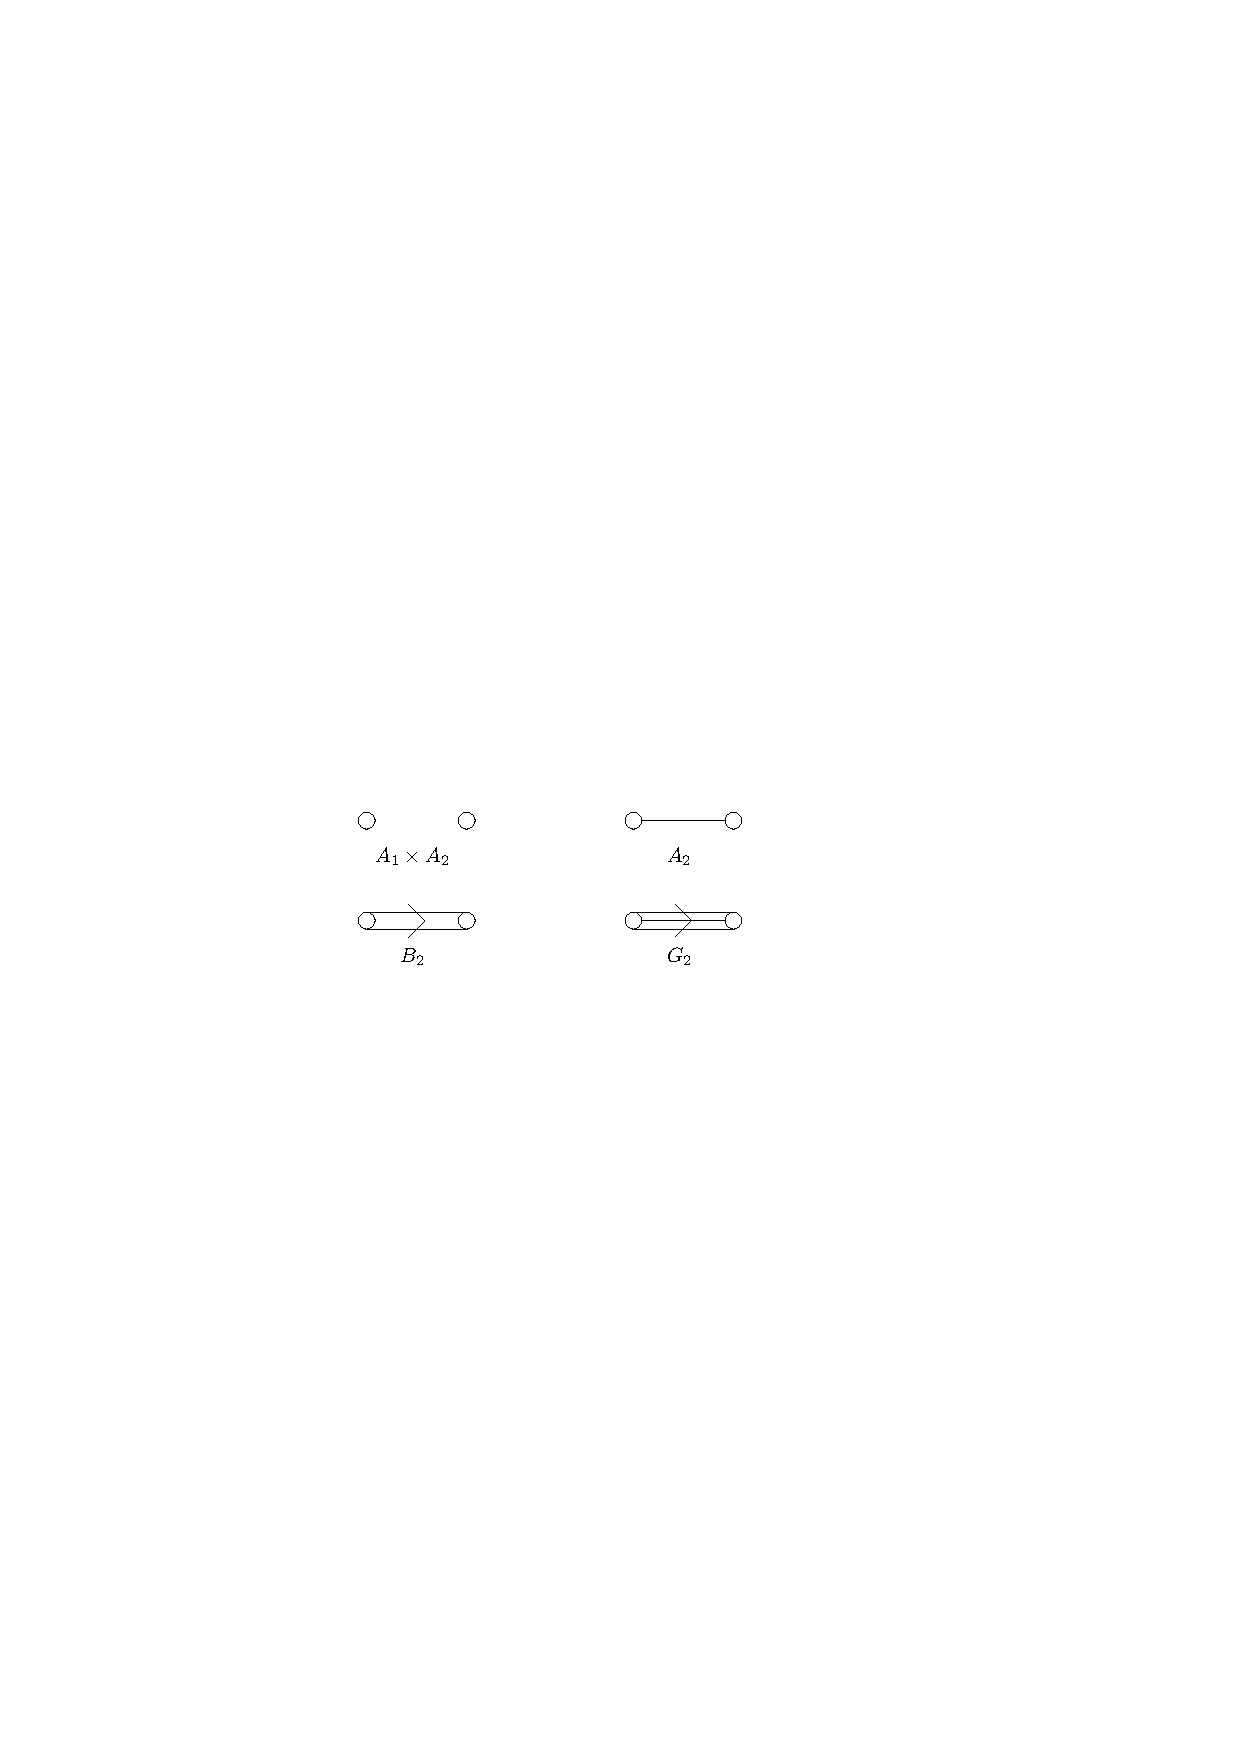
\includegraphics[scale=1]{figures/Dynkin diagrams for the rank-two root systems.pdf}
	\end{figure}
	
	\item 注意, 夹角为 $\frac{2 \pi}{3}, \frac{3 \pi}{4}$ 的根长度一定不相等, 即, $2, 3$ 条线上一定有箭头;相反, 一条线上一定没有箭头.
	
	\item 同一个 root system 的两个 $\Delta_1, \Delta_2$ 的 Dynkin 图一定完全相同 (isomorphic).
	
	\begin{tcolorbox}[title=proof:]
		there exists $w \in W$ s.t. $w[\Delta_1] = \Delta_2$, and $w$ preserves angles and lengths.
	\end{tcolorbox}
	
	\noindent\rule[0.5ex]{\linewidth}{0.5pt} % horizontal line
	
	\item a root system is irreducible (see section \ref{7.1}) $\iff$ its Dynkin diagram is connected.
	\begin{itemize}
		\item semisimple Lie algebra $\mathfrak{g}$ is \textbf{simple} $\iff$ the Dynkin diagram of $R \subset i \mathfrak{t}$ is \textbf{connected}.
	\end{itemize}
	
	\begin{tcolorbox}[title=proof:]
		如果 $R$ 是 reducible, 那么 $\Delta = \Delta_1 \cup \Delta_2$ 且 $\Delta_1 \perp \Delta_2$, 则 Dynkin 图一定 not connected.
		
		\noindent\rule[0.5ex]{\linewidth}{0.5pt} % horizontal line
		
		反之, Dynkin 图 not connected $\Longrightarrow \Delta = \Delta_1 \cup \Delta_2$ 且 $\Delta_1 \perp \Delta_2$, 那么 $E = E_1 \oplus E_2$ with $E_i = \mathrm{span}(\Delta_i)$.
		
		Weyl 群由 $s_\alpha, \alpha \in \Delta$ 生成, 而 $s_\alpha, \alpha \in \Delta_1$ 在 $E_2$ 上是单位映射, 可见 $W = W_1 \times W_2$, 因此, $R = W[\Delta] = W_1[\Delta_1] \cup W_2[\Delta_2] = R_1 \cup R_2$, 即根要么属于 $E_1$ 要么属于 $E_2$.
	\end{tcolorbox}
	
	\item Dynkin diagrams are isomorphic $\iff$ root systems are isomorphic.
\end{itemize}

\section{integral and dominant integral elements}
\begin{itemize}
	\item \textbf{def.:} an element $\mu \in E$ is an \textbf{integral element} if for all $\alpha \in R$,
	\begin{equation}
		\braket{\mu, H_\alpha} = 2 \frac{\braket{\mu, \alpha}}{\braket{\alpha, \alpha}} \in \mathbb{Z}
	\end{equation}
	$\mu$ is \textbf{dominant} (relative to $\Delta$) if $\braket{\mu, \alpha} \geq 0, \forall \alpha \in \Delta$, and \textbf{strictly dominant} if $\braket{\mu, \alpha} > 0, \forall \alpha \in \Delta$.
	\begin{itemize}
		\item $\mu$ is (strictly) dominant (relative to $\Delta_C$) $\iff \mu \in \bar{C}$ (or $C$).
		
		\item for all $\mu$, there exists $w \in W$ s.t. $w \ket{\mu} \in \bar{C}$.
		
		\item every integer linear combination of roots (e.g. $2 \alpha + 3 \beta + 5 \gamma$) is an integral element. 但一般不是所有 integral elements 都是根的整数线性组合.
	\end{itemize}
	
	\item 注意 $\{H_\alpha | \alpha \in \Delta\}$ 是 $R^\vee$ 的 base (见 section \ref{7.4}), 所以 $\braket{\mu, H_\alpha} \in \mathbb{Z}, \forall \alpha \in \Delta \Longrightarrow \mu$ 是 integral element.
	
	\item \textbf{def.:} the \textbf{fundamental weights} (relative to $\Delta = \{\alpha_1, \cdots, \alpha_l\}$) are $\mu_1, \cdots, \mu_r$ s.t.,
	\begin{equation}
		\braket{\mu_i, H_{\alpha_j}} = \delta_{i j}
	\end{equation}
	i.e. the dual basis of $\Delta^\vee$.
	\begin{itemize}
		\item $\Delta^{\vee *}$ 的非负 (正) 整数的线性组合是 (strictly) dominant integral element.
		
		\item $\Delta^{\vee *}$ 的整数线性组合的集合 $=$ integral elements 的集合.
	\end{itemize}
	
	\item \textbf{def.: half the sum of the positive roots} (relative to $\Delta$) is,
	\begin{equation}
		\delta = \frac{1}{2} \sum_{\alpha \in R^+} \alpha
	\end{equation}
	
	\item $\delta$ is a strictly dominant integral element, and,
	\begin{equation}
		\braket{\delta, H_\alpha} = 1, \forall \alpha \in \Delta \iff \delta = \sum_{i = 1}^r \mu_i
	\end{equation}
	
	\begin{tcolorbox}[title=proof:]
		注意 section \ref{7.5} 最后一个定理, $s_\alpha[R^+ - \{\alpha\}] = R^+ - \{\alpha\}$, 所以 $R^+ - \{\alpha\} = \{\beta_1, s_\alpha \beta_1, \beta_2, s_\alpha \beta_2, \cdots\}$. 且有 $\braket{\beta_1 + s_\alpha \beta_1, H_\alpha} = 0$, 所以,
		\begin{equation}
			\braket{\delta, H_\alpha} = \braket{\frac{1}{2} \alpha, H_\alpha} = 1
		\end{equation}
	\end{tcolorbox}
	
	\item fundamental wights and half the sum of the positive roots in rank-two systems 见下图,
	
	\begin{figure}[H]
		\centering
		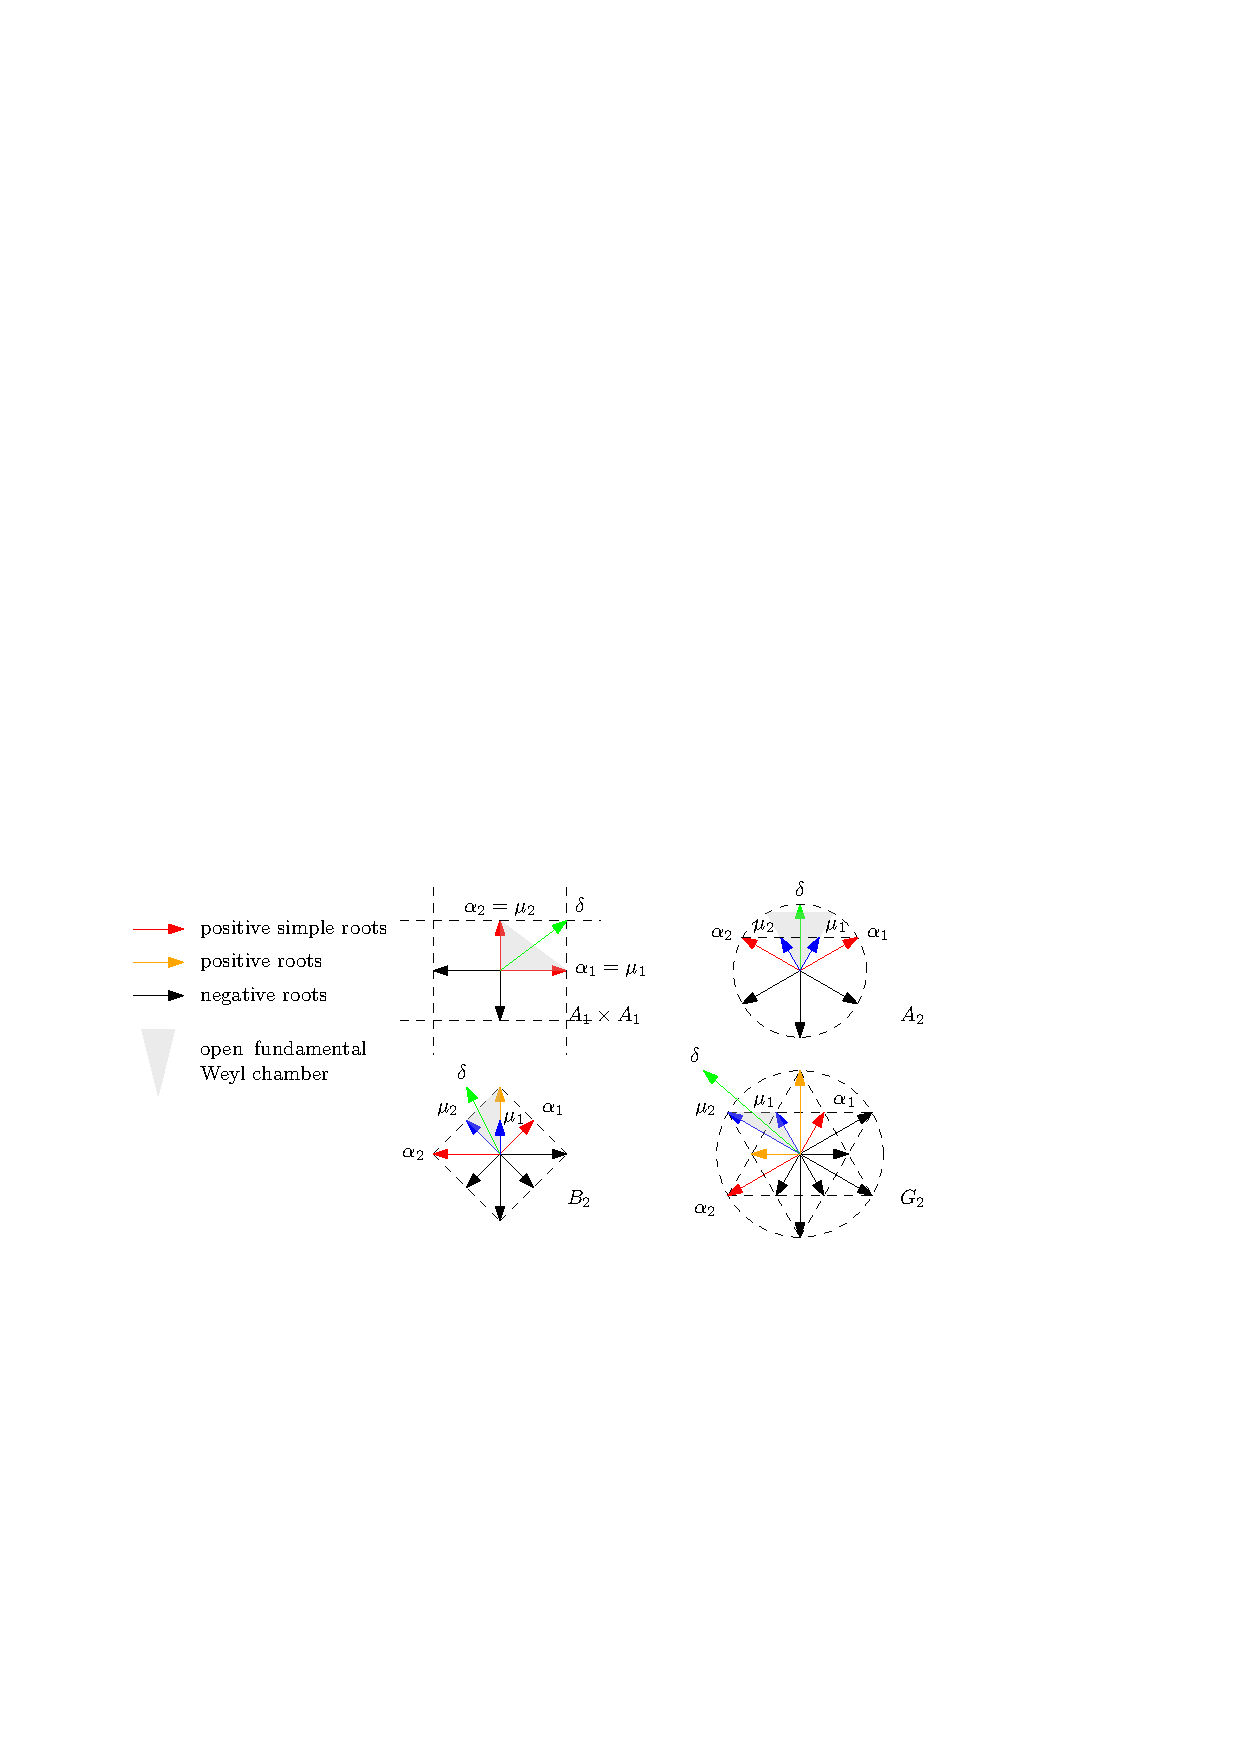
\includegraphics[scale=1]{figures/fundamental wights and half the sum of the positive roots in rank-two systems.pdf}
	\end{figure}
\end{itemize}

\section{the partial ordering} \label{7.8}
\begin{itemize}
	\item \textbf{def.:} relative to $\Delta = \{\alpha_1, \cdots, \alpha_r\}$, $\mu \succeq \nu$ ($\mu$ is \textbf{higher} than $\nu$) if,
	\begin{equation}
		\mu - \nu = c_1 \alpha_1 + \cdots + c_r \alpha_r
	\end{equation}
	其中 $c_1, \cdots, c_r \geq 0$, 类似地, 可以定义 $\nu \preceq \mu$ (... \textbf{lower} than...).
	\begin{itemize}
		\item $\succeq$ 定义了一个 partial ordering on $E$, 但两个矢量之间可能既不存在 $\succeq$ 也不存在 $\preceq$ 的关系.
	\end{itemize}
	
	\noindent\rule[0.5ex]{\linewidth}{0.5pt} % horizontal line
	
	\item $\mu \in E$ is dominant $\Longrightarrow \mu \succeq 0$.
	
	\begin{tcolorbox}[title=proof:]
		考虑 $\Delta$ 的 dual basis $\Delta^* = \{\alpha_1^*, \cdots, \alpha_r^*\}$, 有,
		\begin{equation}
			c_i = \braket{\alpha_i^*, \mu} = \sum_{j = 1}^r \braket{\alpha_i^*, \alpha_j^*} \braket{\alpha_j, \mu}
		\end{equation}
		$\Delta$ 中的任何两个向量夹钝角 (见 section \ref{7.4} 定义后的第一条定理), 那么它的对偶基底中的任意两个向量夹锐角 (见 appendix \ref{A.4}), 所以 $\braket{\alpha_i^*, \alpha_j^*} \geq 0, \braket{\alpha_j, \mu} \geq 0$, 所以 $c_i \geq 0$.
	\end{tcolorbox}
	
	\item if $\mu$ is dominant (i.e. $\mu \in \bar{C}$), then $w \ket{\mu} \preceq \mu$ for all $w \in W$.
	
	\begin{tcolorbox}[title=proof:]
		$O$ is the Weyl-group orbit of $\mu$. 考虑到 $O$ 是有限集合, 令 $\nu \in O$ 使得没有其它元素高于 $\nu$, 那么一定有 $\nu \in \bar{C}$ (即 dominant), 否则, 如果 $\braket{\nu, \alpha} < 0, \exists \alpha \in \Delta_C$, 那么,
		\begin{equation}
			s_\alpha \ket{\nu} = \nu - 2 \frac{\braket{\nu, \alpha}}{\braket{\alpha, \alpha}} \alpha \succeq \nu
		\end{equation}
		考虑到 section \ref{7.5} 的第四个结论, 可知 $\nu = \mu$.
		
		\noindent\rule[0.5ex]{\linewidth}{0.5pt} % horizontal line
		
		现在证明 $O$ 中没有元素既不高于也不低于 $\mu$.
		
		考虑所有既不... 也不... 的元素的集合 $O'$, $\xi \in O'$ 且没有 $O'$ 中的元素高于它, 那么,
		\begin{itemize}
			\item 如果 $o \in O - O'$, 那么一定有 $\mu \succeq o$, 且如果 $o \succeq \xi$, 那么 $\mu \succeq o \succeq \xi$, 与 $\xi \in O'$ 矛盾.
		\end{itemize}
		所以 $O$ 中没有元素高于 $\xi$, 可知 $\xi \in \bar{C}$, 矛盾.
	\end{tcolorbox}
	
	\item if $\mu$ is a strictly dominant ($\mu \in C$) integral element, then $\mu \succeq \delta$ ($\delta$ is half the sum of positive roots).
	
	\begin{tcolorbox}[title=proof:]
		$\mu$ is a strictly dominant integral element $\Longrightarrow \braket{\mu, \alpha} \in \mathbb{Z}^+ - \{0\}, \forall \alpha \in \Delta_C$; $\braket{\delta, \alpha} = 1, \forall \alpha \in \Delta_C$. 所以 $\mu - \delta \in \bar{C} \Longrightarrow \mu \succeq \delta$.
	\end{tcolorbox}
	
	\noindent\rule[0.5ex]{\linewidth}{0.5pt} % horizontal line
	
	\item \textbf{def.:} the \textbf{convex hull} of vectors $v_1, \cdots, v_N$ is the set,
	\begin{equation}
		\mathrm{Conv}(v_1, \cdots, v_N) = \{c_1 v_1 + \cdots + c_N v_N | c_1 + \cdots + c_N = 1 \ \text{and} \ c_i \in \mathrm{R}^+\}
	\end{equation}
	
	两个例子如下图,
	
	\begin{figure}[H]
		\centering
		\subfigure{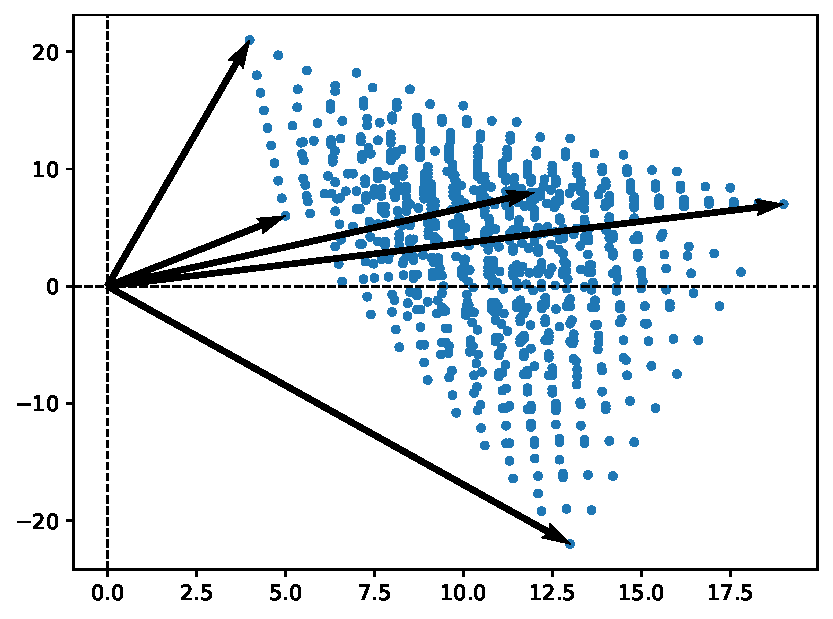
\includegraphics[scale=0.5]{figures/convex hull (1).pdf}} 
		\subfigure{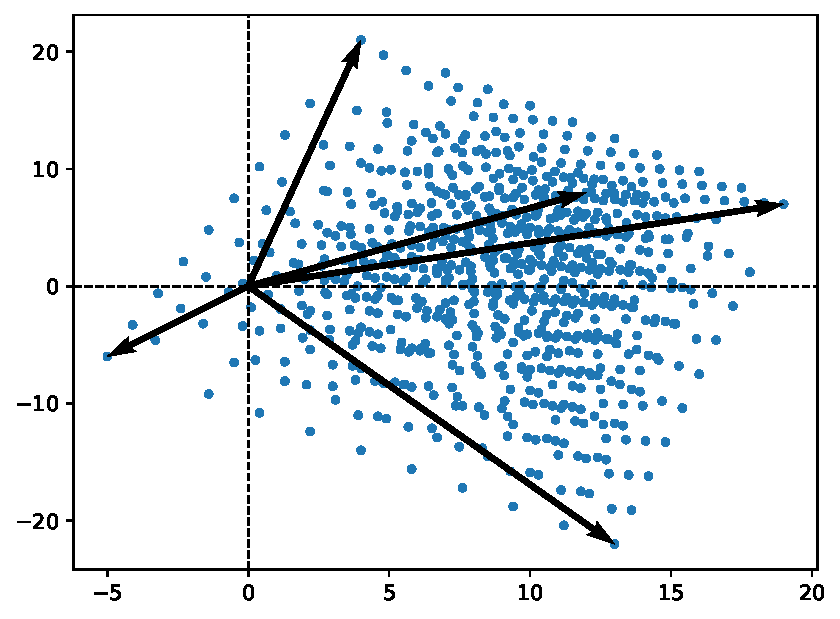
\includegraphics[scale=0.5]{figures/convex hull (2).pdf}}
	\end{figure}
	
	\begin{itemize}
		\item $K$ is a compact, convex subset of $E$, and $\lambda \in E - K$, then there is an element $\gamma \in E$ s.t.,
		\begin{equation}
			\braket{\gamma, \lambda} > \braket{\gamma, \kappa}, \forall \kappa \in K
		\end{equation}
		
		\begin{tcolorbox}[title=proof:]
			由于 $K$ 是紧致的, 存在 $\kappa_0 \in K$ 使得 $|\lambda - \kappa_0|$ 最小, 令 $\gamma = \lambda - \kappa_0$, 那么,
			\begin{equation}
				\braket{\gamma, \lambda - \kappa_0} > 0 \Longrightarrow \braket{\gamma, \lambda} > \braket{\gamma, \kappa_0}
			\end{equation}
			对于 $K$ 中的任意元素 $\kappa$, $\kappa(s) = s \kappa + (1 - s) \kappa_0, s \in [0, 1]$ 属于 $K$, 那么,
			\begin{equation}
				|\lambda - \kappa(s)|^2 \geq |\lambda - \kappa_0|^2 \Longrightarrow s^2 |\kappa - \kappa_0|^2 - 2 s \braket{\lambda - \kappa_0, \kappa - \kappa_0} \geq 0
			\end{equation}
			考虑 $s \ll 1$ 的情况, 可见,
			\begin{equation}
				\braket{\underbrace{\lambda - \kappa_0}_{= \gamma}, \kappa - \kappa_0} \leq 0 \Longrightarrow \braket{\gamma, \lambda} > \braket{\gamma, \kappa_0} \geq \braket{\gamma, \kappa}
			\end{equation}
		\end{tcolorbox}
		
		\item $\mu, \nu$ are dominant ($\in \bar{C}$) and $\nu \notin \mathrm{Conv}(W \ket{\mu})$, then there exists a dominant element $\gamma \in \bar{C}$ s.t.,
		\begin{equation}
			\braket{\gamma, \nu} > \braket{\gamma, w \mu}, \forall w \in W
		\end{equation}
		meaning that $\nu \npreceq w \mu, \forall w \in W$.
		
		\begin{tcolorbox}[title=proof:]
			根据上一个定理, 存在 $\gamma' \in E$ 使得 $\braket{\gamma', \nu} > \braket{\gamma', \kappa}, \forall \kappa \in \mathrm{Conv}(W \ket{\mu})$, 特别地, $\braket{\gamma', \nu} > \braket{\gamma', w \mu}, \forall w \in W$.
			
			考虑 $\{\gamma\} = W \ket{\gamma'} \cap \bar{C}$, 这个 $\gamma = w_0 \gamma'$ 是唯一的, 且 $\gamma \succeq \gamma'$. 所以,
			\begin{equation}
				\gamma - \gamma' \in \bar{C} \Longrightarrow \braket{\gamma - \gamma', \nu} \geq 0 \Longrightarrow \braket{\gamma, \nu} > \braket{w_0 \gamma, w \mu}, \forall w \in W \Longrightarrow \cdots
			\end{equation}
			($\gamma - \gamma'$ 与 positive simple root 的内积为正, 且 $\nu$ 可以展开成 positive simple root 的正系数叠加)
		\end{tcolorbox}
	\end{itemize}
	
	\noindent\rule[0.5ex]{\linewidth}{0.5pt} % horizontal line
	
	\item 两个定理:
	\begin{itemize}
		\item if $\mu, \nu$ are dominant, then $\nu \in \mathrm{Conv}(W \ket{\mu}) \iff \nu \preceq \mu$.
		
		\item $\mu$ is dominant and $\nu \in E$, then $\nu \in \mathrm{Conv}(W \ket{\mu}) \iff w \ket{\nu} \preceq \mu, \forall w \in W$.
	\end{itemize}
	
	\begin{tcolorbox}[title=proof:]
		上一个定理已经证明了 $\Longleftarrow$, 我们现在来证明 $\Longrightarrow$. $\mu$ 是 dominant, 那么 $w \mu \preceq \mu, \forall w \in W$, 所以,
		\begin{equation}
			\Big( \sum_{i = 1}^{|W|} c_i w_i \ket{\mu} \Big) - \mu = \sum_{i = 1}^{|W|} c_i (\underbrace{w_i \ket{\mu} - \mu}_{\preceq 0}) \preceq 0
		\end{equation}
		所以 $\mathrm{Conv}(W \ket{\mu}) \preceq \mu$.
		
		\noindent\rule[0.5ex]{\linewidth}{0.5pt} % horizontal line
		
		首先, 显然有 $\nu \in \mathrm{Conv}(W \ket{\mu}) \iff w \ket{\nu} \in \mathrm{Conv}(W \ket{\mu}), \forall w \in W$. 那么考虑 $\nu' = w_0 \nu \in \bar{C}$, 有,
		\begin{equation}
			\nu \in \mathrm{Conv}(W \ket{\mu}) \iff \nu' \in \mathrm{Conv}(W \ket{\mu}) \iff \nu' \preceq \mu
		\end{equation}
		而 $w \ket{\nu} \preceq \nu' \preceq \mu, \forall w \in W$, 得证.
	\end{tcolorbox}
\end{itemize}

\section{rank-three systems}
\begin{itemize}
	\item 本 section 只考虑 irreducible rank-three systems, 总共有三种, 分别是 $A_3, B_3, C_3$, 它们分别来自 $\mathfrak{sl}(4, \mathbb{C})$, $\mathfrak{so}(7, \mathbb{C})$ 和 $\mathfrak{sp}(3, \mathbb{C})$.
	
	\item $A_3$ root system 见下图, 其中, base 由红色向量组成, Weyl 群是右图中绿色正四面体的对称群,
	
	\begin{figure}[H]
		\centering
		\subfigure{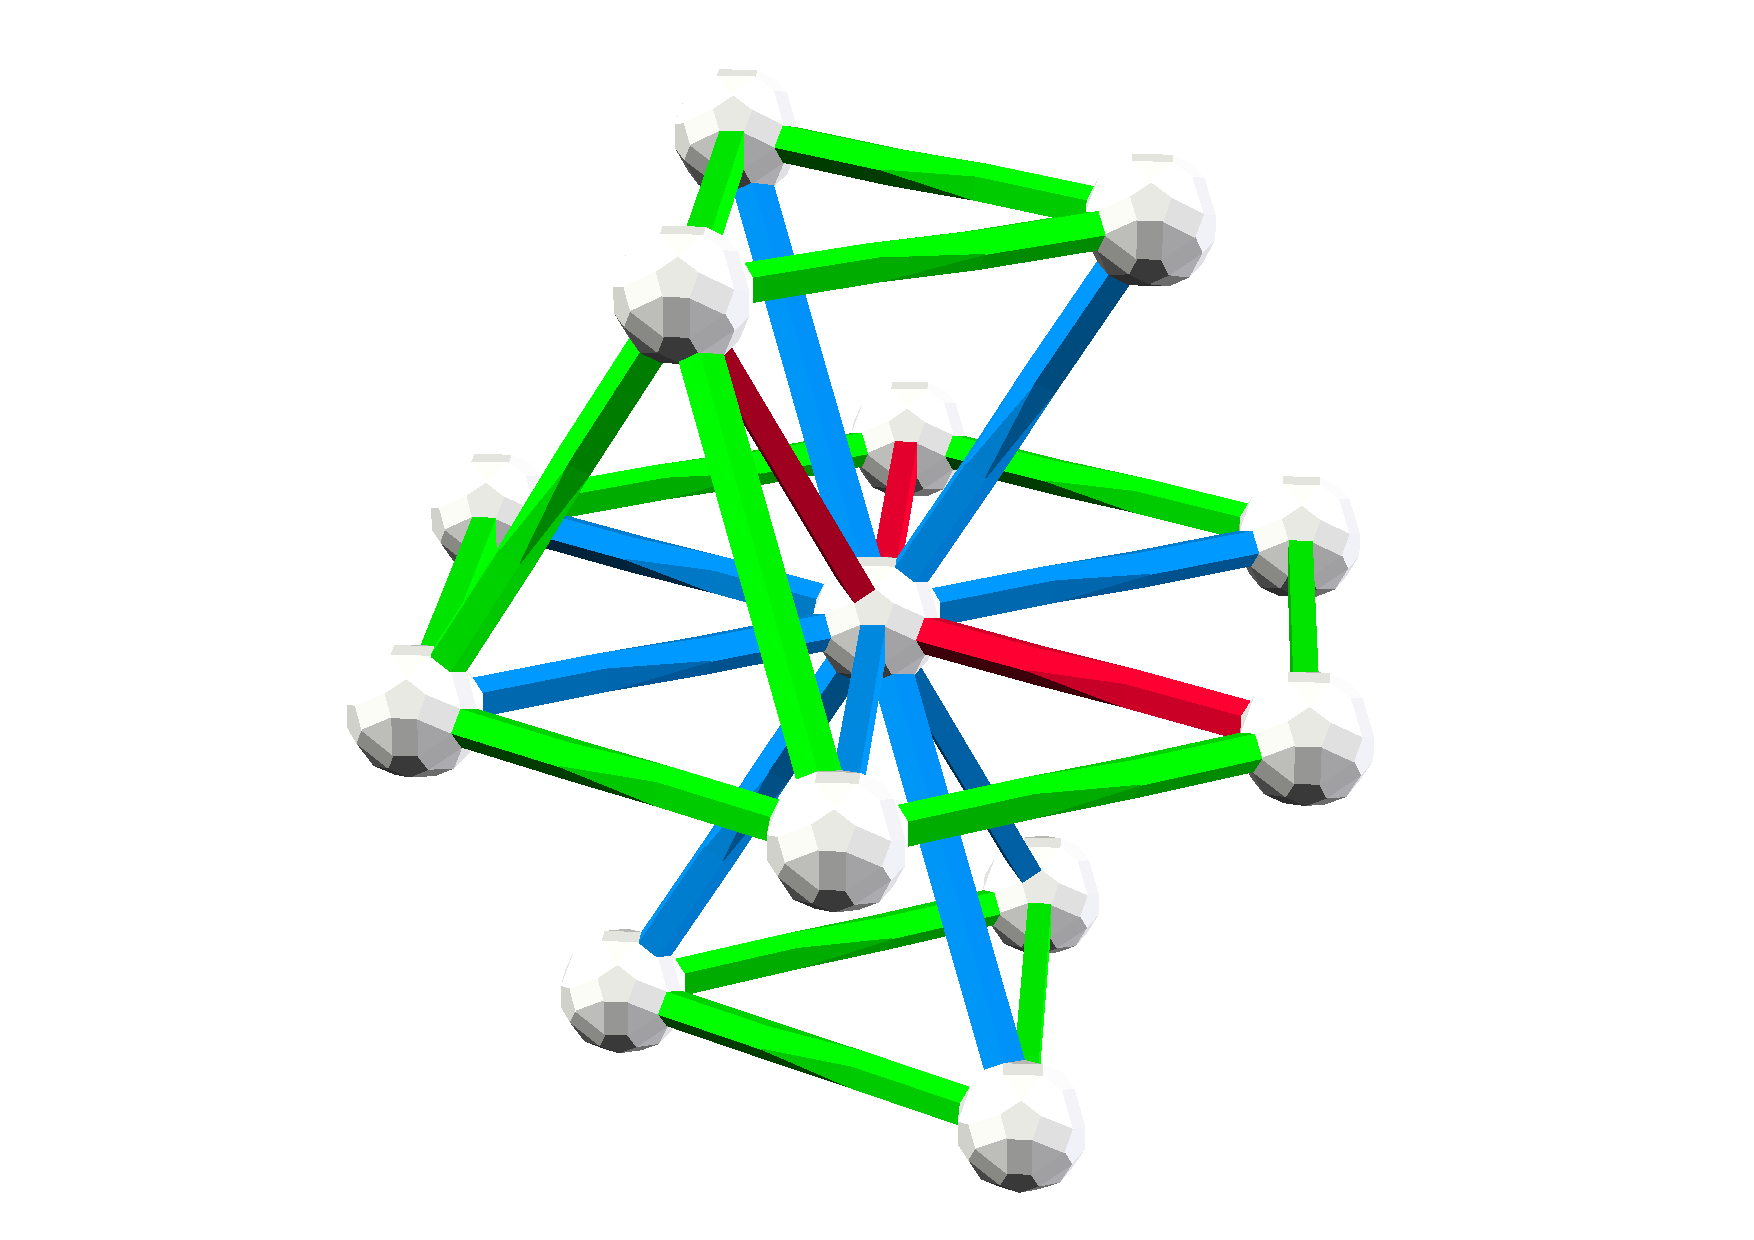
\includegraphics[scale=0.2]{figures/the A3 root system.pdf}}
		\subfigure{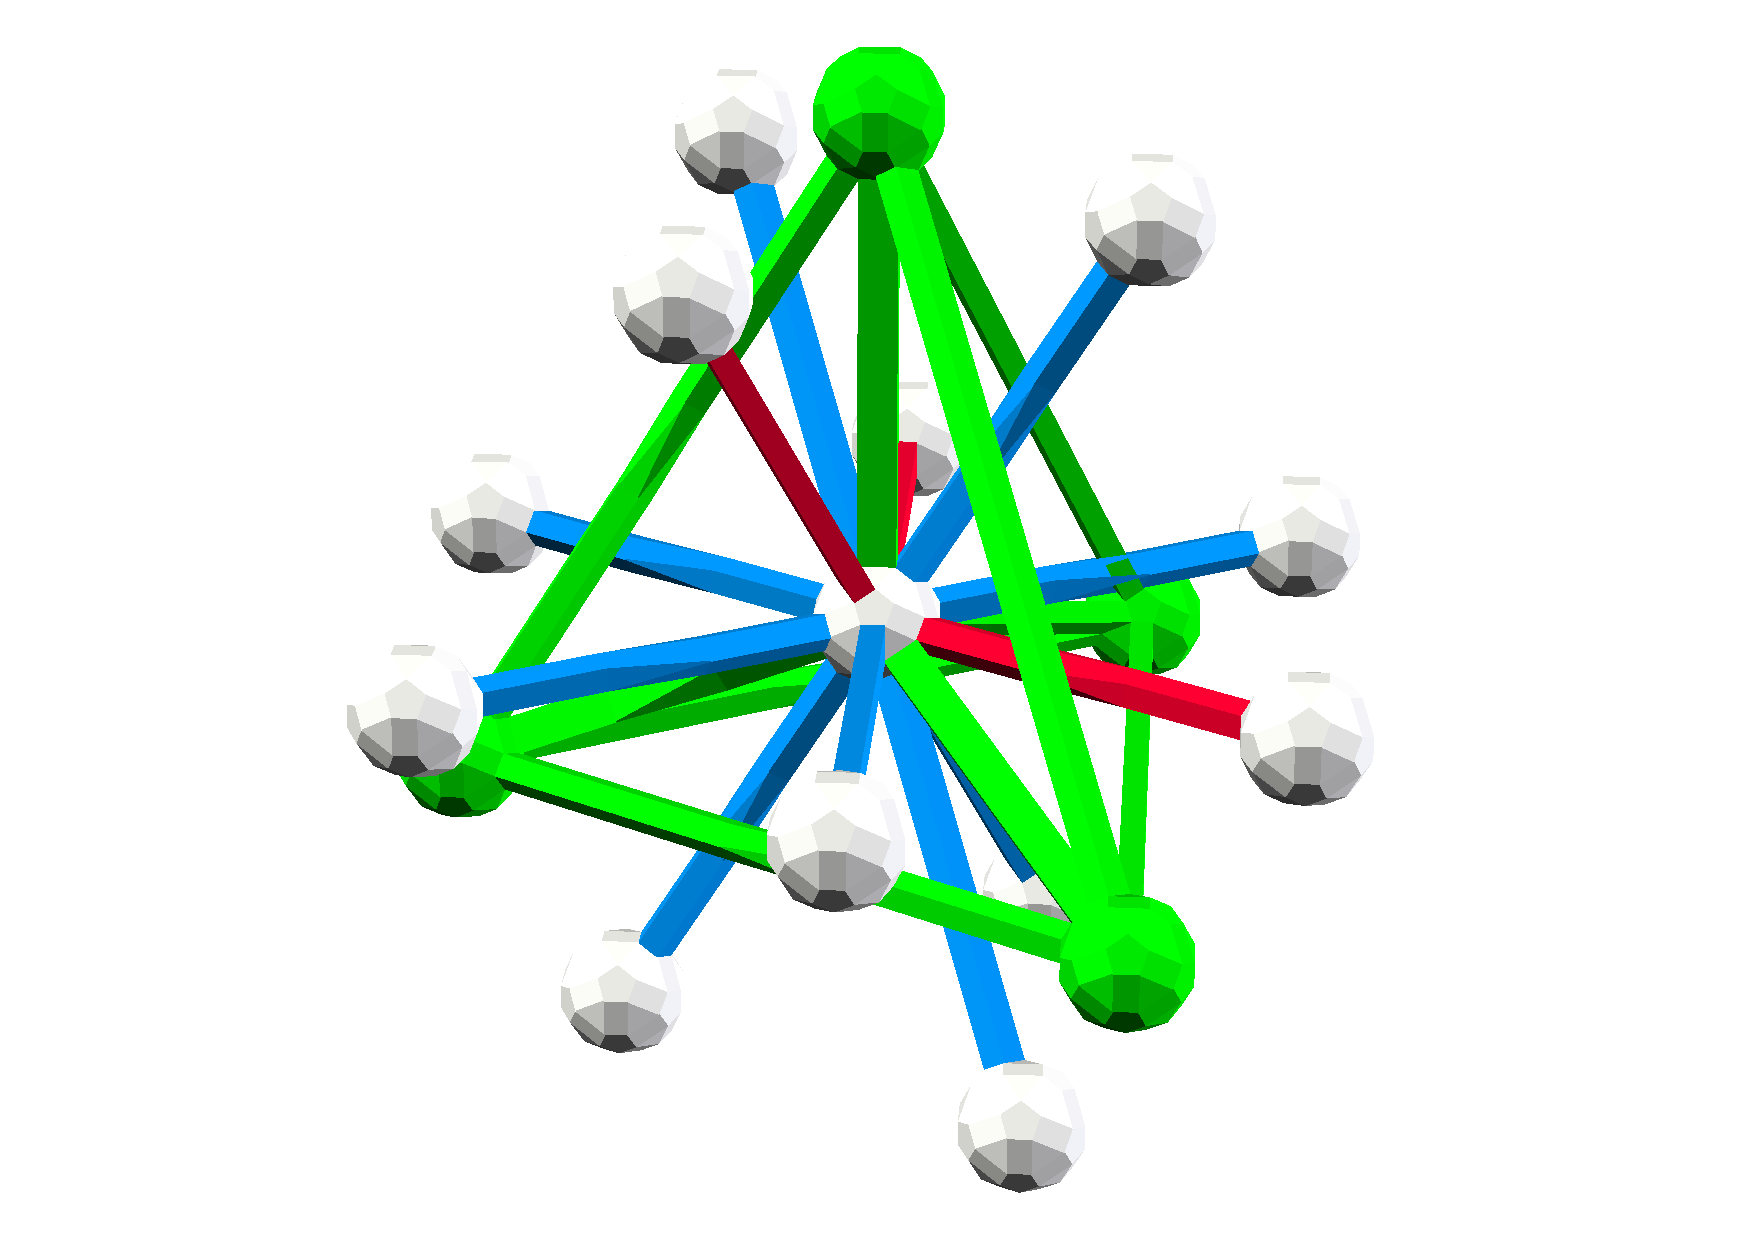
\includegraphics[scale=0.2]{figures/the Weyl group of A3.pdf}}
	\end{figure}
	
	\item $B_3, C_3$ root systems 分别见下图,
	
	\begin{figure}[H]
		\centering
		\subfigure{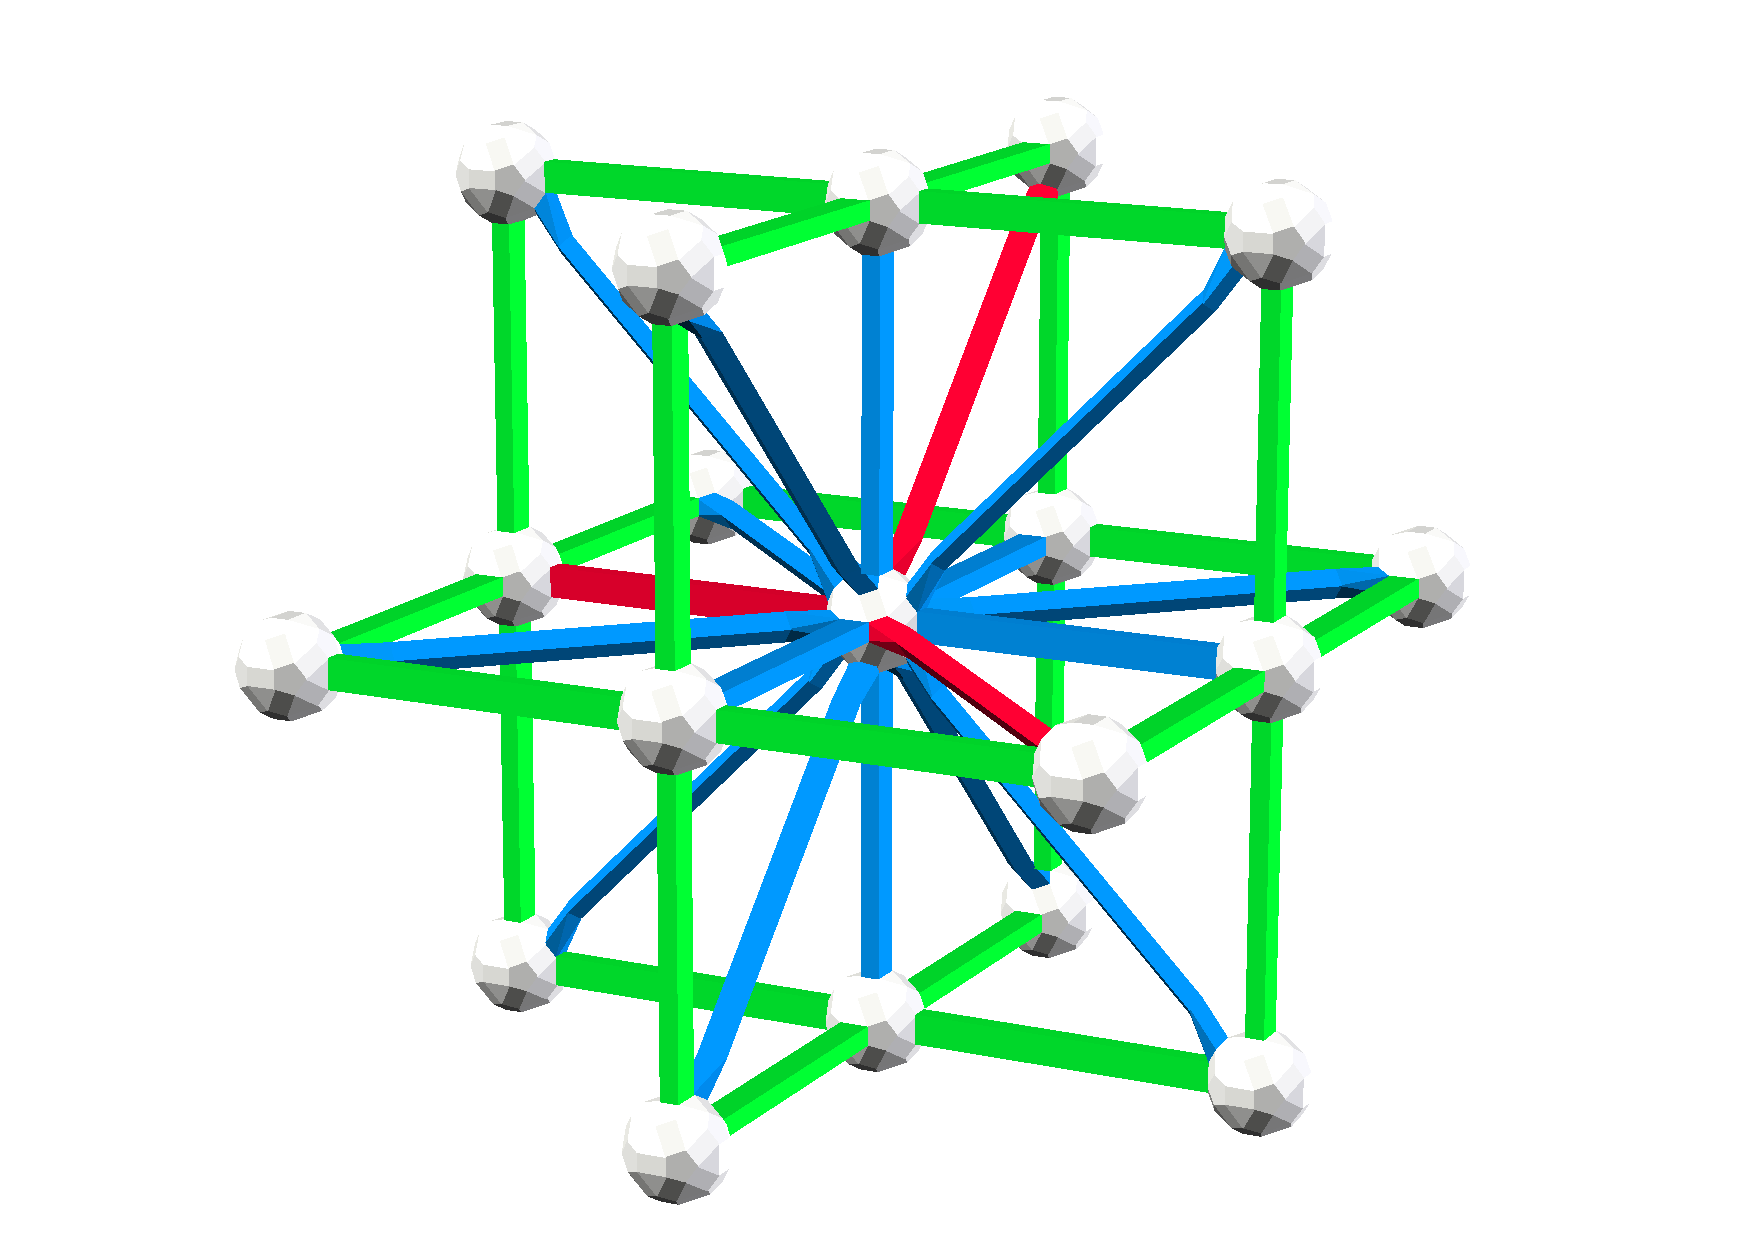
\includegraphics[scale=0.2]{figures/the B3 root system.pdf}}
		\subfigure{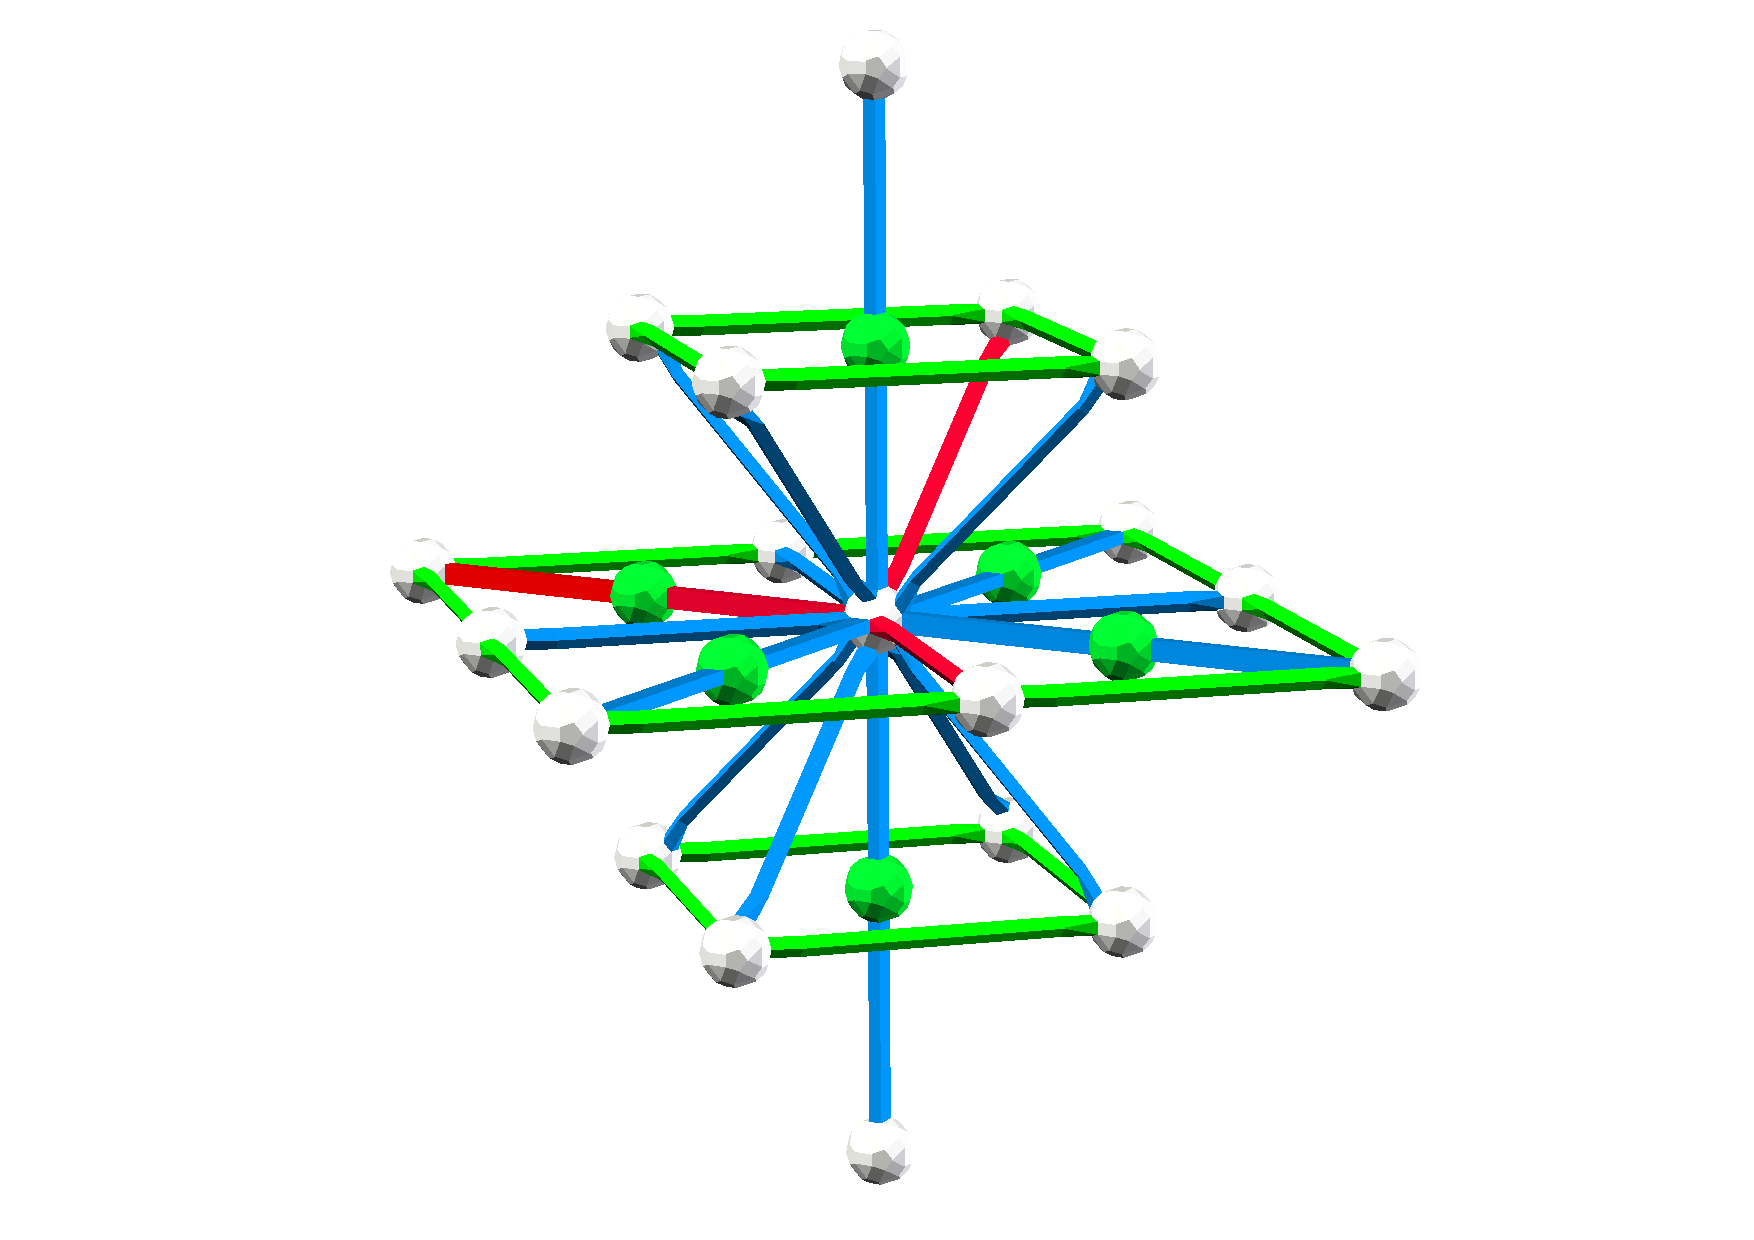
\includegraphics[scale=0.2]{figures/the C3 root system.pdf}}
	\end{figure}
	
	它们的 Weyl 群显然相同, 是下图中黄色立方体的对称群,
	
	\begin{figure}[H]
		\centering
		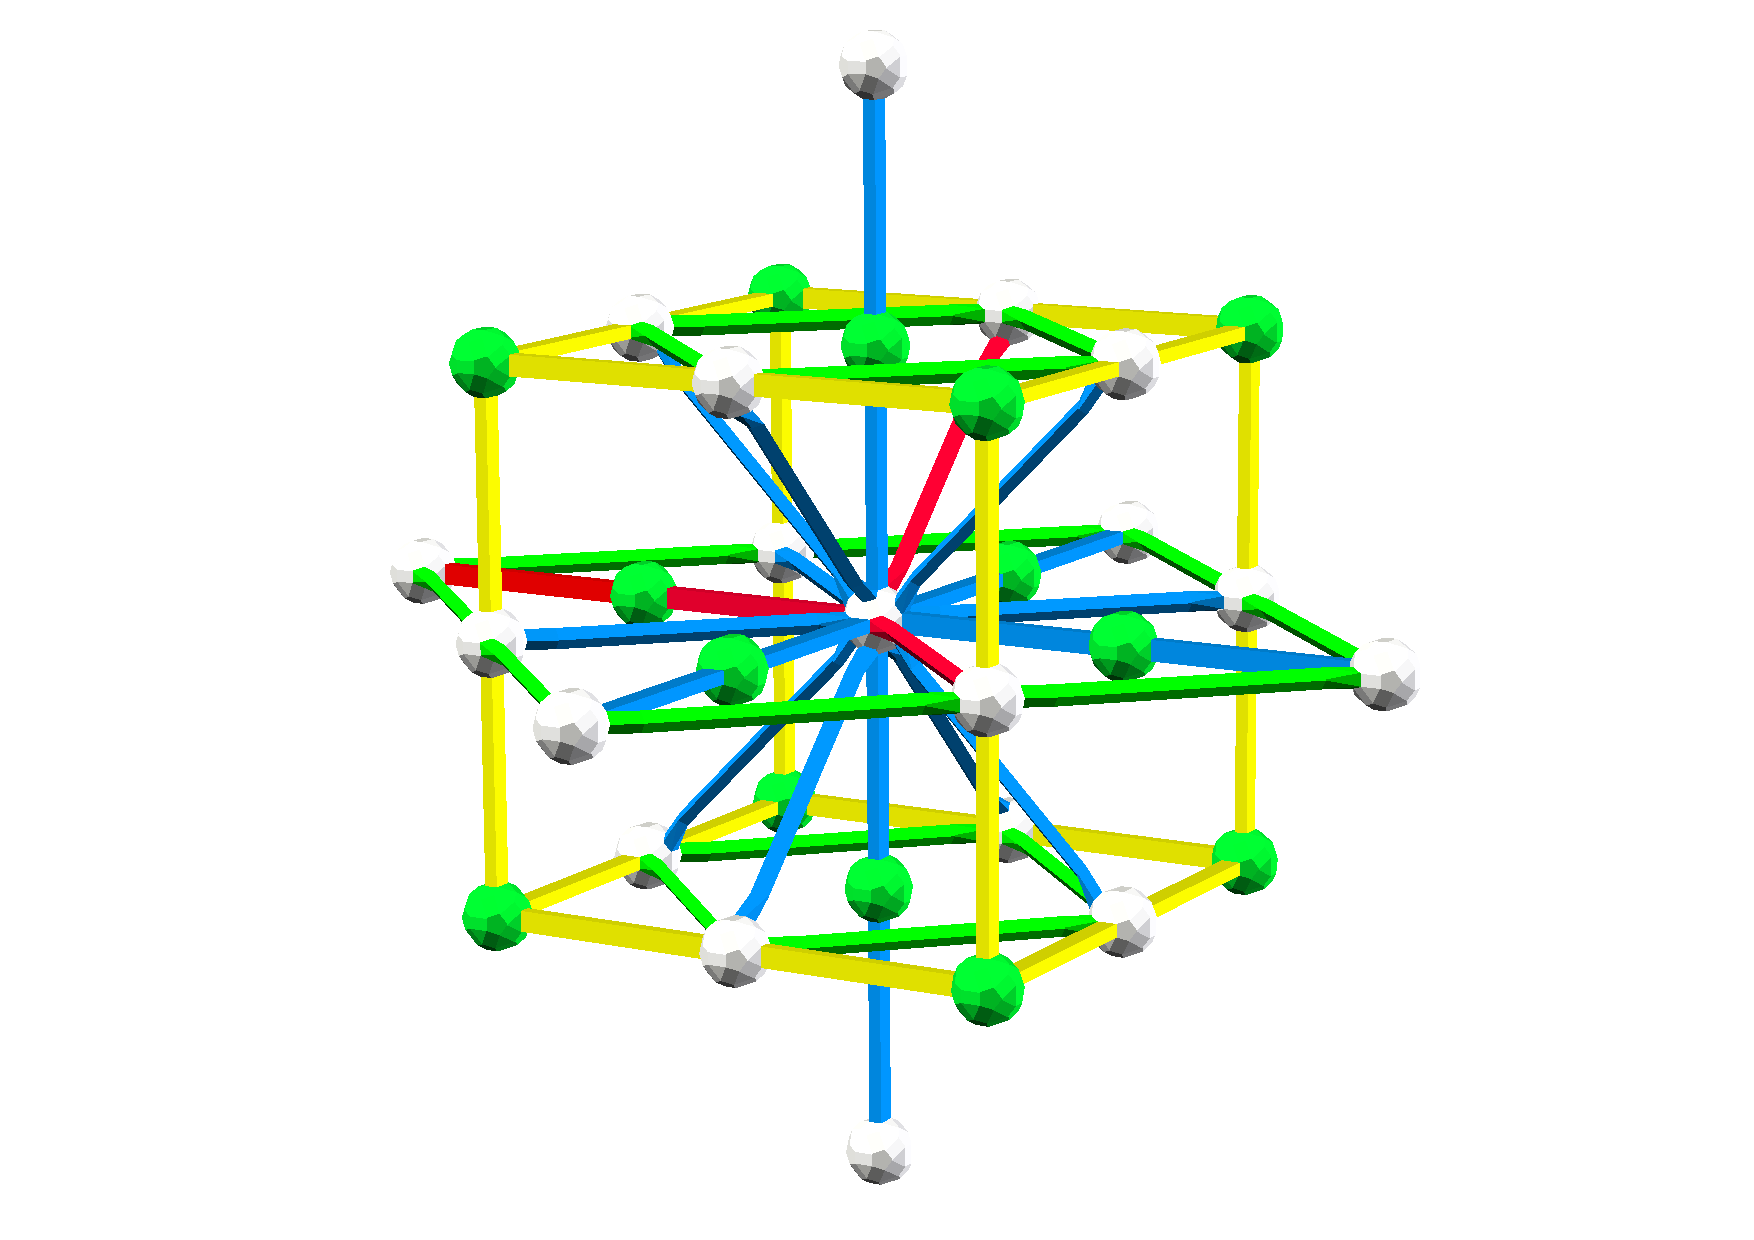
\includegraphics[scale=0.2]{figures/the Weyl group of C3.pdf}
	\end{figure}
\end{itemize}

\section{the classical root systems}
\begin{itemize}
	\item 见 section \ref{6.7}.
\end{itemize}

\section{the classification}
\begin{itemize}
	\item every irreducible root system is either the root system of a classical Lie algebra(types $A_n, B_n, C_n, n \geq 1$ and $D_n, n \geq 3$, with $B_2 \simeq C_2, A_3 \simeq D_3$) or one of five \textbf{exceptional root systems}.
	
	\item the \textbf{exceptional root systems} are $G_2, F_4, E_6, E_7, E_8$, 它们的 Dynkin 图如下,
	
	\begin{figure}[H]
		\centering
		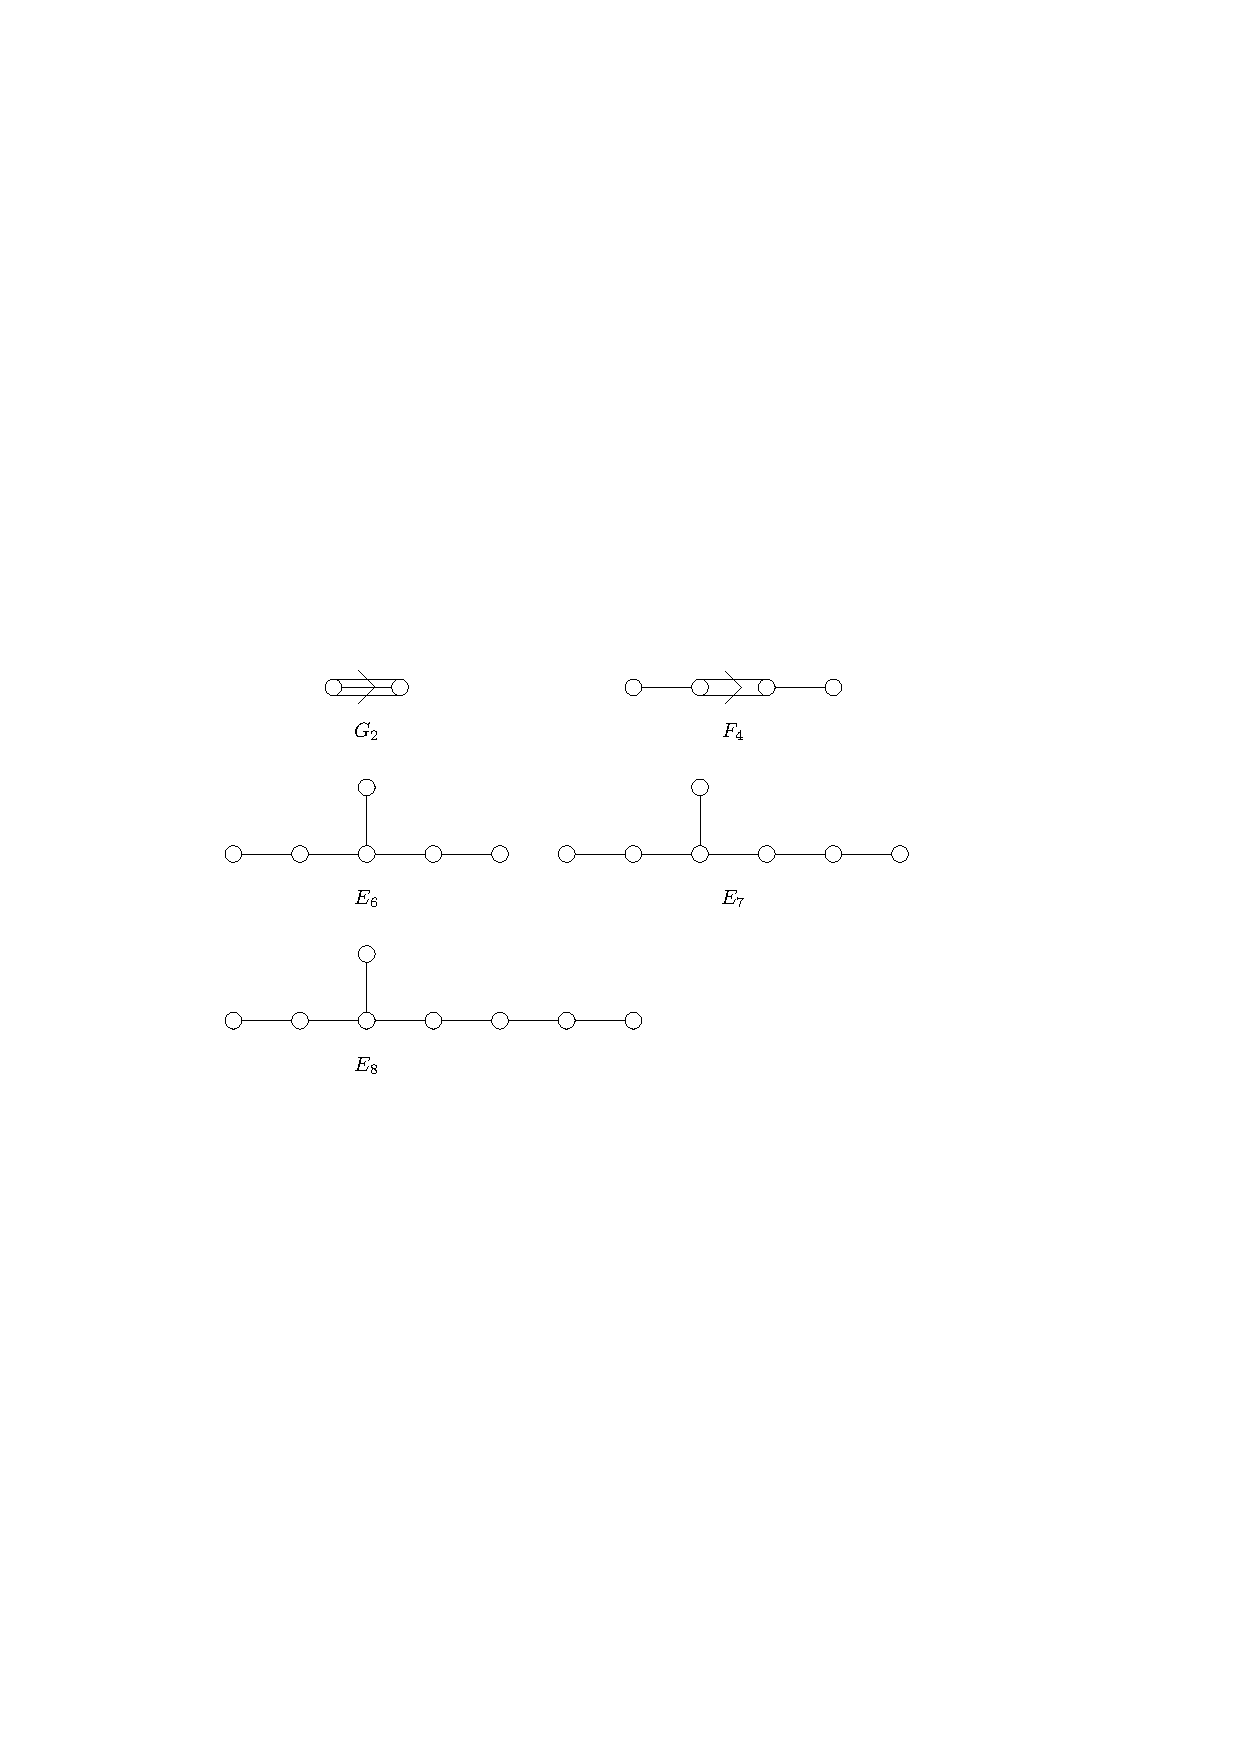
\includegraphics[scale=1]{figures/exceptional Dynkin diagrams.pdf}
	\end{figure}
	
	\item 三个有用的定理:
	\begin{itemize}
		\item $\mathfrak{h}_1, \mathfrak{h}_2$ are Cartan subalgebras of the semisimple Lie algebra $\mathfrak{g}$, then there exists a automorphism (自同构) $\phi : \mathfrak{g} \rightarrow \mathfrak{g}$ s.t. $\phi[\mathfrak{h}_1] = \mathfrak{h}_2$. (见 section \ref{6.2} 末尾)
		
		\item the root systems associated to $(\mathfrak{g}_1, \mathfrak{h}_1)$ and $(\mathfrak{g}_2, \mathfrak{h}_2)$ are isomorphic $\Longrightarrow \mathfrak{g}_1, \mathfrak{g}_2$ are isomorphic.
		
		\item for every root system $R$, there exists a root system associated to $(\mathfrak{g}, \mathfrak{h})$ isomorphic to $R$.
	\end{itemize}
	因此, 所有 simple Lie algebra 都与下表中的某个 classical Lie algebra,
	\begin{center}
		\newcolumntype{K}{>{\centering\arraybackslash}X}
		\begin{tabularx}{\linewidth}{KKKK}
			\toprule
			$\mathfrak{sl}(n + 1, \mathbb{C}) \mapsto A_n$ & $\mathfrak{so}(2 n + 1, \mathbb{C}) \mapsto B_n$ & $\mathfrak{sp}(2 n, \mathbb{C}) \mapsto C_n$ & $\mathfrak{so}(2 n, \mathbb{C}) \mapsto D_n$ \\
			\midrule
			$n \geq 1$ & $n \geq 2$ & $n \geq 3$ & $n \geq 4$ \\
			\midrule
			\multicolumn{1}{c|}{$n = 1$} & \multicolumn{1}{c}{$B_1 \simeq A_1$} & $C_1 \simeq A_1$ & $n \neq 1$ \\
			\multicolumn{1}{c|}{$n = 2$} & \multicolumn{1}{c}{} & $C_2 \simeq B_2$ & $n \neq 2$ \\
			\multicolumn{1}{c|}{$n = 3$} & \multicolumn{1}{c}{} &  & $D_3 \simeq A_3$ \\
			\bottomrule
		\end{tabularx}
	\end{center}
	或 $G_2, F_4, E_{6, 7, 8}$ 中的某个 exceptional Lie algebra 相 isomorphic.
\end{itemize}
